\documentclass[]{usiinfbachelorproject}
\usepackage{subfigure, wrapfig, url, array, caption}
\usepackage[ngerman,english]{babel}
\captionsetup{labelfont={bf}}

\author{Raphael Schapfel}

\title{Vectorize Pixel Art}
\subtitle{Transforming bitmaps into SVG}
\versiondate{\today}

\begin{committee}
%With more than 1 advisor an error is raised...: only 1 advisor is allowed!
\advisor[Universit\`a della Svizzera Italiana, Switzerland]{Prof.}{Kai}{Hormann}
%You can comment out  these lines if you don't have any assistant
%\assistant[Universit\`a della Svizzera Italiana, Switzerland]{Title}{AssistantName1}{AssistanSurname1}
%\assistant[Universit\`a della Svizzera Italiana, Switzerland]{Title}{AssistantName2}{AssistanSurname2}
\end{committee}

\abstract {
In this project I implemented an algorithm for extracting a resolution-independent vector representation from pixel art images, based on the paper of Johannes Kopf and Dani Lischinski \cite{Kopf2011}. This algorithm resolves pixel-scale features in the input and converts them into regions separated by piecewise-smooth contour curves. In the original image, a raster graphics image (or bitmap), pixels are distributed in a generally rectangular grid represented by a dot matrix data structure, where diagonal neighbors are only connected through a single point. This causes thin features to become visually disconnected under magnification by conventional means, and creates ambiguities in the connectedness and separation of diagonal neighbors. The key to this algorithm is in resolving these ambiguities and reshape the pixel cells so that neighboring pixels belonging to the same feature are connected through edges, thereby preserving the feature connectivity under magnification. The pixel aliasing artifacts are then reduced and smoothed by fitting spline curves to the contours of the image and smoothing their control points.
}


\begin{document}
\maketitle

%%%%%%%%%%%%%%%%%%%%%%%%%
\section{Introduction} \label{sec:intro} 
%%%%%%%%%%%%%%%%%%%%%%%%%

\subsection{Pixel Art}

Pixel art is a form of digital art where images are build, edited and represented on the pixel level. It is a technique that follows the footsteps of the divisionism (also known as {\it pointillisme}), whose greatest exponent was Georges Seurat (see Figure \ref{fig:seurat}). The divisionism was the characteristic style in Neo-Impressionist painting defined by the separation of colors into individual dots or patches which interacted optically. The most obvious difference is that instead of using a brush, pixel art images are created through the use of a mouse and a raster graphics software.

\begin{figure}[ht]
	\centering
	\subfigure[]{
		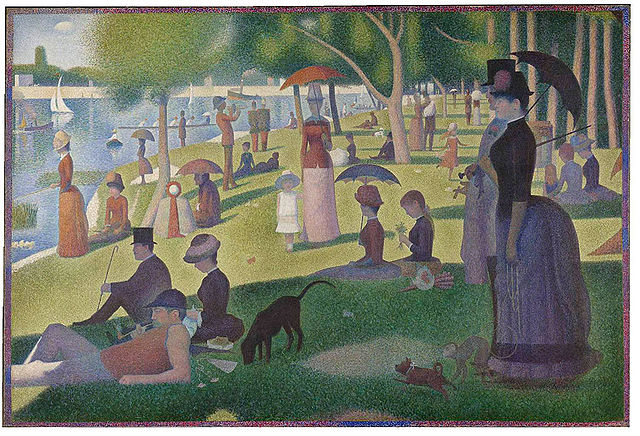
\includegraphics[height=6cm]{img/seurat.jpeg}
		\label{fig:seurat}
	}
	\subfigure[]{
		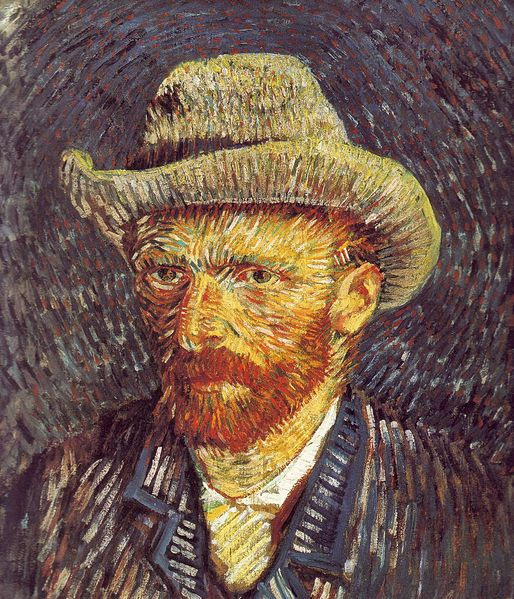
\includegraphics[height=6cm]{img/gogh.jpeg}
		\label{fig:gogh}
	}
	\caption{Famous examples of divisionism painting: \subref{fig:seurat} ``Un dimanche apr\`es-midi \`a l'\^Ile de la Grande Jatte'' (1884-1886) by Georges Seurat and \subref{fig:gogh} ``Self Portrait with felt Hat'' (1887-1888) by Vincent van Gogh.}
	\label{fig:divisionism}
\end{figure}

Graphics in most old (or relatively limited) computer and video games, graphing calculator games, and many mobile phone games are mostly pixel art (see Figure \ref{fig:pixelart}). It was very often used in older computer and console video games before the mid '90s, when this art was created as a necessity: in those years the graphics of video games and computers was simple, the pixels were very large and the images appeared poorly defined. Because of the hardware constraints at the time, artists where forced to work with only a small indexed palette of colors and meticulously arrange every pixel by hand, rather than mechanically downscaling higher resolution artwork. For this reason, classical pixel art is usually marked by an economy of means, minimalism, and inherent modesty, which some say is lost in modern computer graphics. 

\begin{figure}[ht]
	\centering
	\subfigure[]{
		
\includegraphics[height=3cm]{img/jump.png}
		\label{fig:jump}
	}
	\subfigure[]{
		
\includegraphics[height=2.5cm]{img/space.png}
		\label{fig:space}
	}
	\subfigure[]{
		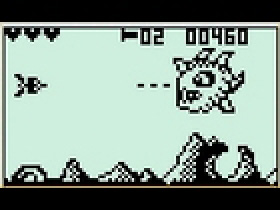
\includegraphics[height=3cm]{img/impact.jpeg}
		\label{fig:impact}
	}
	\subfigure[]{
		
\includegraphics[height=2.5cm]{img/sonic.png}
		\label{fig:sonic}
	}
	\subfigure[]{
		
\includegraphics[height=2.5cm]{img/setup.png}
		\label{fig:setup}
	}
	\caption{Examples of classic pixel art applied to console video-games, computer video-games, mobile phone games and operating systems icons (Input images: \subref{fig:jump} Mario \copyright Nintendo Co., Ltd.; \subref{fig:space} Space Invaders \copyright Taito Corp.; \subref{fig:impact} Space Impact \copyright Nokia Corp.; \subref{fig:sonic} Sonic \copyright Sega Corp.; \subref{fig:setup} Setup icon \copyright Microsoft Corp.)}
	\label{fig:pixelart}
\end{figure}

\subsubsection{Modern applications}

With the increasing use of 3D graphics in games, pixel art lost some of its use. Despite that, it is still a very active professional/amateur area, since mobile phones and other portable devices still have low resolution and therefore require skillful use of space and memory. \\
Modern pixel art has also been seen as a reaction to the 3D graphics industry by amateur game/graphic hobbyists. Many retro enthusiasts often choose to mimic the style of the past in their creations, where they argue that graphics were more aesthetically pleasing.\\
Sometimes pixel art is used for advertising too. One such company that uses pixel art to advertise is Bell. The group \emph{eBoy} specializes in pixel graphics for advertising and has been featured in magazines such as \emph{Wired}, \emph{Popular Science}, and \emph{Fortune 500} (see an example of their amazing work in Figure \ref{fig:eboy}) \cite{Wiki:pixelart}.\\

\begin{figure} [ht]
	\centering
	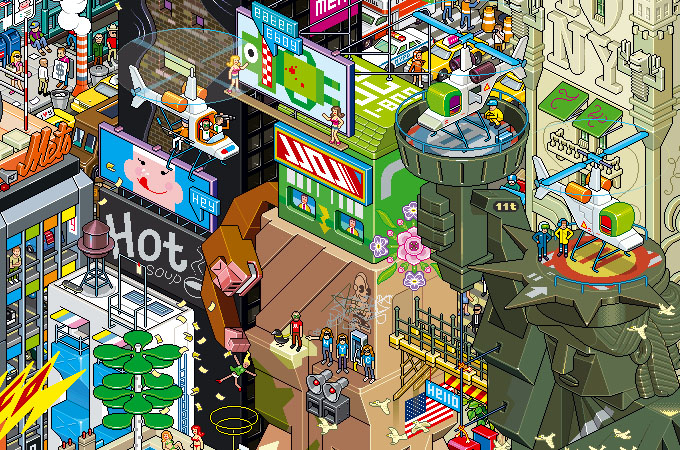
\includegraphics[width=0.9\textwidth]{img/eboy.jpeg}
	\caption{Detail of ``New York'' by eBoy}
	\label{fig:eboy}
\end{figure}

Icons for operating systems with limited graphics abilities are also pixel art. The limited number of colors and resolution presents a challenge when attempting to convey complicated concepts and ideas in an efficient way. On the Microsoft Windows desktop icons are raster images of various sizes, the smaller of which are not necessarily scaled from the larger ones and could be considered pixel art. On the GNOME and KDE desktops, icons are represented primarily by SVG images, but with hand-optimized, pixel art PNGs for smaller sizes such as 16x16 and 24x24 \cite{Wiki:pixelart}. Also favicons are another example of pixel art used on modern desktop computers.\\
Pixel art has been used also in the virtual worlds \emph{Citypixel}, \emph{Minecraft} and \emph{Habbo} as well as among hand-held devices such as the Nintendo DS and the Play Station Portable (PSP) \cite{Wiki:pixelart}.\\
It is therefore, at least in part, a return to simplicity: the pixel reappears and emphasizes the importance that a single point has for these artists, seen as something essential, which in combination with other points forms a much more complex picture.

%%%%%%%%%%%

\subsection{Vector Graphics}

Vector graphics is the use of geometrical primitives such as points, lines, curves, and shapes or polygons, which are all based on mathematical expressions, to represent images in computer graphics. ``Vector'', in this context, implies more than a straight line.
Vector graphics is based on images made up of vectors (also called paths, or strokes) which lead through locations called control points. Each of these points has a definite position on the $x$ and $y$ axes of the work plan. Each point, as well, is a variety of database, including the location of the point in the work space and the direction of the vector (which is what defines the direction of the track). Each track can be assigned a color, a shape, a thickness and also a fill (or gradient). This does not affect the size of the files in a substantial way because all information resides in the structure; it describes how to draw the vector (see left image of Figure \ref{fig:vector_raster}).\\
Raster graphics images on the other hand are produced by digital image capture devices: digital scanners or digital cameras, or by pixel editing programs (e.g., Adobe Photoshop). Raster images are composed of a matrix (grid) or bitmap of digital picture elements (pixels). Pixels are squares or rectangles described as black, white, gray or color (see right image of Figure \ref{fig:vector_raster}).

\begin{figure} [ht]
	\centering
	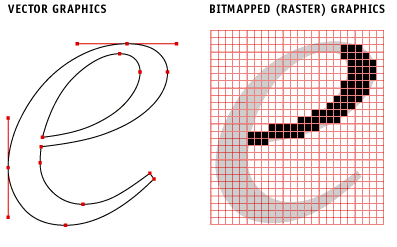
\includegraphics[scale=0.7]{img/vector_raster.png}
	\caption{Difference between vector graphics and raster graphics: in vector graphics images are represented by geometrical primitives (points, lines, curves, etc.) while in raster graphics images are composed by a matrix of pixels.}
	\label{fig:vector_raster}
\end{figure}

Modern displays and printers are raster devices; vector formats have to be converted to raster format (bitmaps -- pixel arrays) before they can be rendered (displayed or printed) (see Section \ref{sec:rasterization}). The size of the bitmap/raster-format file generated by the conversion will depend on the resolution required, but the size of the vector file generating the bitmap/raster file will always remain the same. Thus, it is easy to convert from a vector file to a range of bitmap/raster file formats but it is much more difficult to go in the opposite direction (and often is not possible), especially if subsequent editing of the vector picture is required. It might be an advantage to save an image created from a vector source file as a bitmap/raster format, because different systems have different (and incompatible) vector formats, and some might not support vector graphics at all. However, once a file is converted from the vector format, it is likely to be bigger, and it loses the advantage of scalability without loss of resolution (see Figure \ref{fig:shark}). It will also no longer be possible to edit individual parts of the image as discrete objects.

\begin{figure}[ht]
	\centering
	\subfigure[]{
		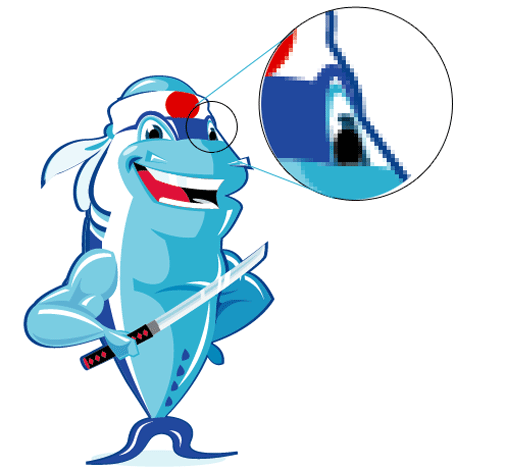
\includegraphics[height=8cm]{img/raster_shark.png}
		\label{fig:rshark}
	}
	\subfigure[]{
		
\includegraphics[height=8.5cm]{img/vector_shark.png}
		\label{fig:vshark}
	}
	\caption{Example showing the effect of raster graphics and vector graphics under magnification: \subref{fig:rshark} raster image magnified 4x and \subref{fig:vshark} vector image magnified 4x. Raster images scale poorly, while vector-based images can be scaled indefinitely without degradation.}
	\label{fig:shark}
\end{figure}

\subsubsection{Rasterization} \label{sec:rasterization}

Rasterization is the task of taking an image described in a vector graphics format and converting it into a raster image for output on a video display or printer, or for storage in a bitmap file format. The term ``rasterization'' can in general be applied to any process by which vector information can be converted into a raster format.
\begin{figure} [ht]
	\centering
	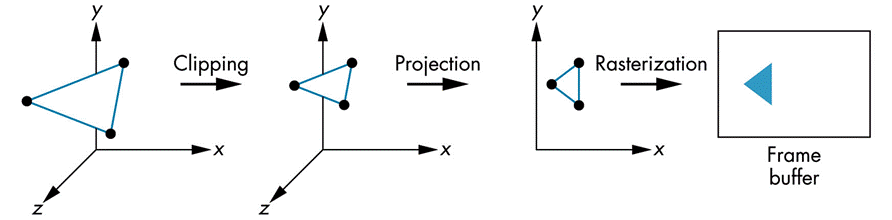
\includegraphics[width=0.8\textwidth]{img/pipeline.png}
	\caption{Classic 3D rasterization pipeline.}
	\label{fig:pipeline}
\end{figure}
\begin{wrapfigure}{r}{0.20\textwidth}
	\centering
	
\includegraphics[width=0.18\textwidth]{img/raster.png}
	\caption{(a) Initial vector shape, (b) black-and-white and (c) greyscale rasterization.}
	\label{fig:rasterization}
\end{wrapfigure}
In normal usage, the term refers to the popular rendering algorithm for displaying three-dimensional shapes on a computer. Rasterization is currently the most popular technique for producing real-time 3D computer graphics, which need to respond immediately to user input, and generally need to produce frame rates of at least 24 frames per second to achieve smooth animation \cite{Wiki:rasterization}.\\
Compared with other rendering techniques such as ray tracing, rasterization is extremely fast. However, rasterization is simply the process of computing the mapping from scene geometry to pixels and does not prescribe a particular way to compute the color of those pixels.\\
The process of rasterizing 3D models onto a 2D plane for display on a computer screen is often carried out by fixed function hardware within the graphics pipeline. This is because there is no motivation for modifying the techniques for rasterization used at render time and a special-purpose system allows for high efficiency.\\
The most basic rasterization algorithm takes a 3D scene, described as polygons, and renders it onto a 2D surface, usually a computer monitor. Polygons are themselves represented as collections of triangles. Triangles are represented by 3 vertices in 3D-space. At a very basic level, rasterizers simply take a stream of vertices, transform them into corresponding 2-dimensional points on the viewer's monitor (following the pipeline in Figure \ref{fig:pipeline}) and fill in the transformed 2-dimensional triangles as appropriate (also known as scan conversion) \cite{Wiki:rasterization} (see Figure \ref{fig:rasterization}).\\
When applied to 2D vector images, rasterization refers only to the final step in the traditional rasterization process: the scan conversion. The scan conversion consists of drawing polygons and vector objects on the raster image, by filling the right pixels with the color determined by the shading. This is equivalent to solving the following two problems: determine the pixels affected by a segment; and determine the points inside the polygon.\\
The classic algorithm to draw a line segment is the Bresenham algorithm (see Figure \ref{fig:bresenham}), which generates a connected sequence of pixels. After drawing a pixel, the algorithm chooses among its 8-neighbors which one to draw according to the line equation, using only integer arithmetic \cite{Wiki:bresenham}.\\
For filling polygons the standard algorithm is called scan-line algorithm (see Figure \ref{fig:scanline}). The polygon is filled by taking a line that scans row by row from the bottom to the top. Each line is then scanned from left to right, and when an edge of the polygon is detected, the successive pixels of the line are drawn until another edge is found \cite{Wiki:scanline}.

\begin{figure}[ht]
	\centering
	\subfigure[]{
		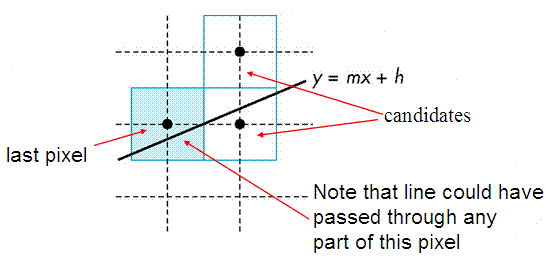
\includegraphics[height=3.9cm]{img/bresenham.png}
		\label{fig:bresenham}
	}
	\subfigure[]{
		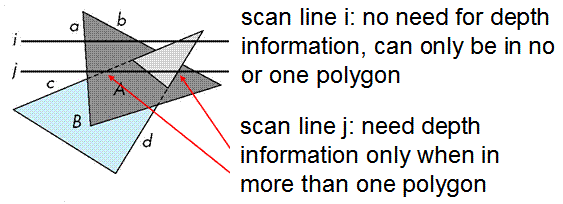
\includegraphics[height=3cm]{img/scanline.png}
  		\label{fig:scanline}
	}
	\caption{Illustrations of \subref{fig:bresenham} the Bresenham algorithm and \subref{fig:scanline} the scan-line algorithm.}
\end{figure}

\subsubsection{Applications}

The earliest 2D computer graphics were all vector graphics. One of the first uses of vector graphic displays was the US SAGE air defense system \cite{Wiki:vector}. Vector graphics systems were only retired from U.S. en route air traffic control in 1999, and are likely still in use in military and specialised systems. Vector graphics were also used on the TX-2 at the MIT Lincoln Laboratory by computer graphics pioneer Ivan Sutherland to run his program Sketchpad in 1963 \cite{Sutherland1963}.\\
Subsequent vector graphics systems, most of which iterated through dynamically modifiable stored lists of drawing instructions, include the IBM 2250, Imlac PDS-1, and DEC GT40. There was a home gaming system that used vector graphics called Vectrex as well as various arcade games like Asteroids and Space Wars. Storage scope displays, such as the Tektronix 4014, could display vector images but not modify them without first erasing the display \cite{Wiki:vector}.

\begin{wrapfigure}{l}{0.42\textwidth}
	\centering
	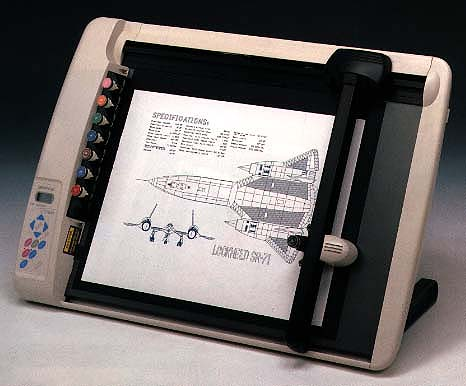
\includegraphics[width=0.41\textwidth]{img/plotter.jpeg}
	\caption{The pen plotter MP5300 from Graphtech.}
	\label{fig:plotter}
\end{wrapfigure} 
\noindent Modern vector graphics displays can sometimes be found at laser light shows, where two fast-moving X-Y mirrors position the beam to rapidly draw shapes and text as straight and curved strokes on a screen.\\
Vector graphics can be created in hardcopy form using a pen plotter, a special type of printer that uses a series of ballpoint and/or felt-tip pens on a servo-driven mount that moves horizontally across the paper, with the plotter moving the paper or the pen back and forth through its paper path for vertical movement (see Figure \ref{fig:plotter}). Although a typical plot might easily require a few thousand paper motions, back and forth, the paper doesn't slip.\\
Present-day vector graphic files such as engineering drawings are typically printed as bitmaps, after vector-to-raster conversion.\\
The term ``vector graphics'' is mainly used today in the context of two-dimensional computer graphics. It is one of several modes an artist can use to create an image on a raster display. Other modes include text, multimedia, and 3D rendering.\\
Most images created with tools such as Adobe Illustrator and CorelDraw are in the form of vector image files. Vector image files are easier to modify than raster image files (which can, however, sometimes be reconverted to vector files for further refinement).\\
Animation images are also usually created as vector files. For example, Shockwave's Flash product lets you create 2D and 3D animations that are sent to a requestor as a vector file and then rasterized ``on the fly'' as they arrive.

\begin{wrapfigure}{r}{0.42\textwidth}
	\centering
	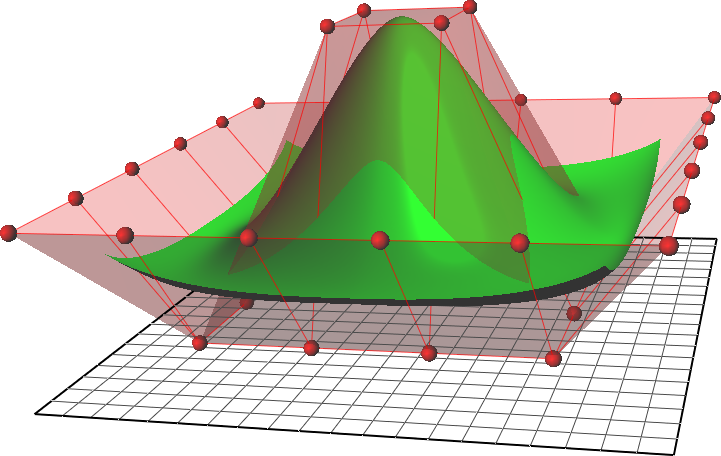
\includegraphics[width=0.41\textwidth]{img/nurbs.png}
	\caption{A three-dimensional NURBS surface.}
	\label{fig:nurbs}
\end{wrapfigure}
\noindent Virtually all modern 3D rendering is done using extensions of 2D vector graphics techniques. In 3D computer graphics, vectorized surface representations are most common (bitmaps can be used for special purposes such as surface texturing, height-field data and bump mapping). At the low-end, simple meshes of polygons are used to represent geometric detail in applications where interactive frame rates or simplicity are important. At the high-end, where one is willing to trade-off higher rendering times for increased image quality and precision, smooth surface representations such as B\'ezier patches, NURBS (see Figure \ref{fig:nurbs}) or Subdivision surfaces are used. One can, however, achieve a smooth surface rendering from a polygonal mesh through the use of shading algorithms such as Phong and Gouraud.

%%%%%%%%%%%

\subsection{Motivation}

\subsubsection{The pixel art appeal} \label{sec:appeal}

In the modern era of fast computers and High Definition screens, the role of pixel as technological device has significantly diminished, yet the use of old pixel graphics as tool of artistic expression in the course of past decade escalated enormously. Today pixel art can be easily found both in and beyond computer screen. 8-bit images present in modern advertising, street graffiti art, music album and magazine covers, digital and print artwork, tattoos and so on. This raises a curious question: how such an old and limited technology enjoys a tremendous degree of popularity in the modern ``hi-tech'' world? I think we can partially find an answer if we look back into the history of arts. In it's nature, pixel graphics is in many ways similar to various traditional art forms, such as embroidery (cross-stitch), mosaic, stained glass and many others types of art where image is constructed out of multiple small colored elements. Even in the last century's expressionistic paintings could be discovered the essence of pixel art (see Figure \ref{fig:divisionism}). \\
The beauty of pixel graphics is that it is representational and abstract at the same time, it's expressive power lies in its ambiguity and simplicity. Nowadays many people view 8-bit graphics as a creative answer to the modern 3D graphic industry with it's strive for complexity and photorealism, and argue that graphics were visually more pleasing in second and third generation consoles \cite{website:nostalgia}.\\
Most importantly, it is undeniable that the golden age of console games left a significant cultural imprint on the society and peoples past. As childhood experience generally plays an important part in any artists work, many graphic designers tend to nostalgically return to that retro image of '80s to recapture the spirit of ``good old times''. The best pixel art from the '80s and '90s video games are masterpieces, many of which have become cultural icons that are instantly recognized by a whole generation, e.g. ``Space Invaders'' or the 3-color Super Mario Bros. sprite (see Figure \ref{fig:pixelart}). These video games continue to be enjoyed today, thanks to numerous emulators that were developed to replace hardware that has long become extinct. For artists and their fans, that nostalgia continues to be a huge part of pixel art's appeal. In the rapidly changing world of technology, pixel art represents a reminder of simpler times. \\
Plus, pixel art is inherently shareable and format-friendly. Because the pixel is, by nature, digital, the art form lends itself perfectly to web culture. And a lot of people think that those works are cool because they see the amount of work put into it \cite{website:nostalgia}.\\
For artists, pixels are pleasurable to work with. One strong trait of pixel art is that it drives the artist to find levels of abstraction. And there's something very satisfying in transforming an idea or an object into an abstract interpretation. Pixels and blocks are really good at this, they are highly modular and very, very easy to handle and understand.\\
EBoy is modern proof that pixel art is thriving. The company caters to a wide swath of geek culture, one that not only celebrates retro pixel technology, but can also appreciate new pixel iterations. After all, the pixel is not static. Artists can work with pixels of many shapes and sizes, can arrange them in infinite types of grids, and can adapt them according to the tastes of different age groups. That's one reason pixel art has been able to reach across the generations. But in the end, pixel fandom remains strongest among the people who grew up alongside the technology. Pixel art has that nerdic old school charm. A lot of people between 30 and 40 like that style because it reminds them of the good old times. Pixel art is the most communicative and most abstract art form easily available to games, and it comes with bonus nostalgia points \cite{website:arstechnica}.\\

We know now that pixel art revival is a need and aspiration shared by many, and this leads us to the first motivation behind the project, which lies in a simple question: how can pixel art still be enjoyed today as it was in the past years? \\
Many techniques have been developed to allow classic low resolution images and games to be more visually appealing on modern HD displays, most of which are described in Section \ref{sec:state} and implement in different ways an \emph{image scaling} method \cite{Wiki:scaling}. In computer graphics, \emph{image scaling} is the process of resizing a digital image, which is a non-trivial process that involves a trade-off between efficiency, smoothness and sharpness. As the size of an image is increased, so the pixels which comprise the image become increasingly visible, making the image appear blurry and ``edgy''. Conversely, reducing an image will tend to enhance its smoothness and apparent sharpness.\\
Typically, image size is decreased (or subsampled or downsampled) in order to produce thumbnails or to fit a smaller display area. Enlarging an image (upsampling or interpolating) is generally common for making smaller imagery fit a bigger screen in fullscreen mode. In ``zooming'' an image, it is not possible to discover any more information in the image than already exists, and image quality inevitably suffers. However, there are several methods of increasing the number of pixels that an image contains, which evens out the appearance of the original pixels.\\
When pixel art is displayed at a higher resolution than the source image, it is often scaled using the nearest-neighbor interpolation algorithm. This avoids blurring caused by other algorithms, such as bilinear and bicubic interpolation--which interpolate between adjacent pixels and work best on continuous tones, but not sharp edges or lines (see Figure \ref{fig:nonadaptive}). Nearest-neighbor interpolation preserves these sharp edges, but it makes diagonal lines and curves look blocky, an effect called pixelation \cite{Wiki:scaling}. Thus, hybrid algorithms have been devised to interpolate between continuous tones while preserving the sharpness of lines in the piece; such attempts include the 2xSaI, Super Eagle, and the high-quality hqx algorithms (see Section \ref{sec:state}) \cite{Wiki:pixelart}.\\
Even though many specialized pixel art upscaling methods have been developed in the previous decade, and can often produce commendable results, due to their local nature the results suffer from stair-casing artifacts, and the algorithms are often unable to correctly resolve locally-ambiguous pixel configurations. Furthermore, the magnification factor in all these methods is fixed to 2$\times$, 3$\times$, or 4$\times$.\\
My goal in this project is to overcome these limitations, by resolving connectivity ambiguities and reshape the pixel cells so that neighboring pixels belonging to the same feature are connected through edges. To allow for custom magnification and preserve the image features I chose to follow a vectorization technique, which converts bitmaps into vector graphics and has many advantages over raster based techniques.

%%%%%%%%%%%

\subsubsection{Vector graphics vs. raster graphics}

Converting pixel art into vector graphics leads to the same benefits that come with any vector based image:
\begin{itemize}
	\item \textbf{Lightweight}: such a system of description of graphic information features the undoubted advantage of a greater data compression: in practice, this minimal amount of information translates to a much smaller file size compared to large raster images. The size of the representation is based on the complexity of the image and the number of graphic elements it contains, rather than the image size or the color depth. 
	\item \textbf{Resolution independent}: vector drawings can be scalable to any size without any loss in quality or resolution. Moreover, the dimensions in device-independent units are usually specified, which results in the best possible rasterization on raster devices.
	\item \textbf{Object oriented}: vector images are made up of many individual, scalable objects (lines, curves, and shapes with editable attributes such as color, fill, and outline). This means that moving, scaling, rotating, filling etc. doesn't degrade the quality of a drawing since the parameters of objects are stored and can be later modified.
	\item \textbf{Programmable}: vector images can be easily generated, modified and animated by programs and scripts, since they are described by mathematical descriptions of objects.
	\item \textbf{Realistic}: from a 3D perspective, rendering shadows is also much more realistic with vector graphics, as shadows can be abstracted into the rays of light from which they are formed. This allows for photo realistic images and renderings (see Figures \ref{fig:leica} and \ref{fig:phone}).
	\item \textbf{Human friendly}: the data is expressed in a form directly understandable by a human being (e.g. the SVG standard). A person can act directly on the image even without using any graphics software or even without detailed knowledge about it. For example, to translate the text of an SVG image it's often enough to open the file with a text editor and modify the lines in the file.
\end{itemize}
\begin{wrapfigure}[22]{r}{0.52\textwidth}
 	\centering
	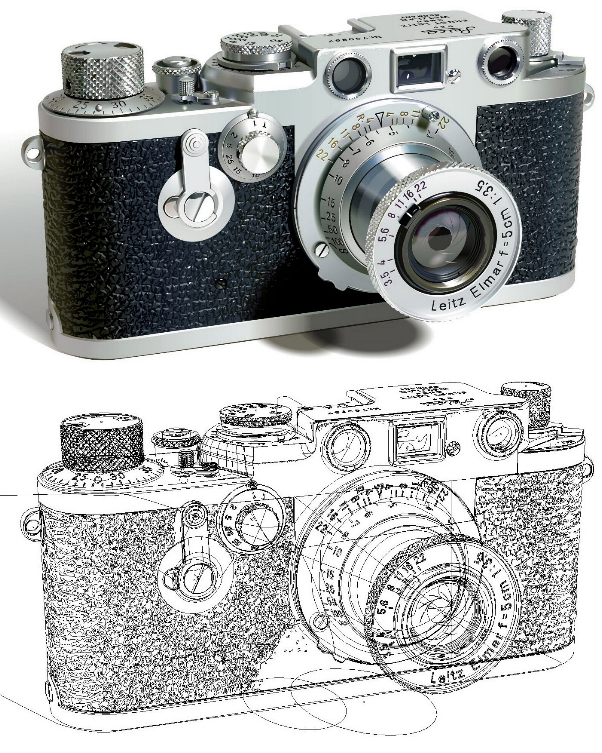
\includegraphics[width=0.5\textwidth]{img/leica.png}
  	\caption{Photorealistic vector art from Yukio Miyamoto.}
	\label{fig:leica}
\end{wrapfigure}

\noindent The problem with vectorization techniques until now is that they were designed for natural images and are based on segmentation and edge detection filters that do not resolve well the tiny features present in pixel art. These methods typically group many pixels into regions, and convert the regions' boundaries into smooth curves. However, in pixel art, every single pixel can be a feature on its own or carry important meaning. As a result, previous vectorization algorithms typically suffer from detail loss when applied to pixel art inputs.\\
This brings us to the second motivation for this project: implement a vectorization technique able to preserve the details at the single pixel level. The fact that every pixel was manually placed causes pixel art to carry a maximum of expression and meaning per pixel. \\
While the quantized nature of pixel art provides for a certain aesthetic in its own right, I believe that a compelling vector art that manages to capture some of the charm of the original might be a very intriguing and ambitious goal.

\newpage 

%%%%%%%%%%%%%%%%%%%%%%%%%
\section{State of the Art} \label{sec:state}
%%%%%%%%%%%%%%%%%%%%%%%%%

The previous work related to this project can be classified into three categories:
\begin{itemize}
	\item {\bf \ref{sec:imageup} General image upsampling (or interpolation)}: essentially these techniques work by using known data to estimate values at unknown points;
	\item {\bf \ref{sec:pixelartup} Pixel art upscaling techniques}: since they are typically used to improve the appearance of earlier video games on arcade and console emulators, most are designed to run in real time for sufficiently small input images and work only on specific scale factors (2$\times$, 3$\times$ and 4$\times$);
	\item {\bf \ref{sec:imagevect} Image vectorization}: the process of converting raster graphics into vector graphics, which is resolution independent.
\end{itemize}

\begin{figure}[ht]
	\centering
	\subfigure[Nearest-neighbor (4$\times$)]{
		
\includegraphics[width=0.45\textwidth]{img/dolphin.png}
		\label{fig:dolphin}
	}
	\subfigure[PhotoZoom Pro 4 (General Image Upsampling)]{
		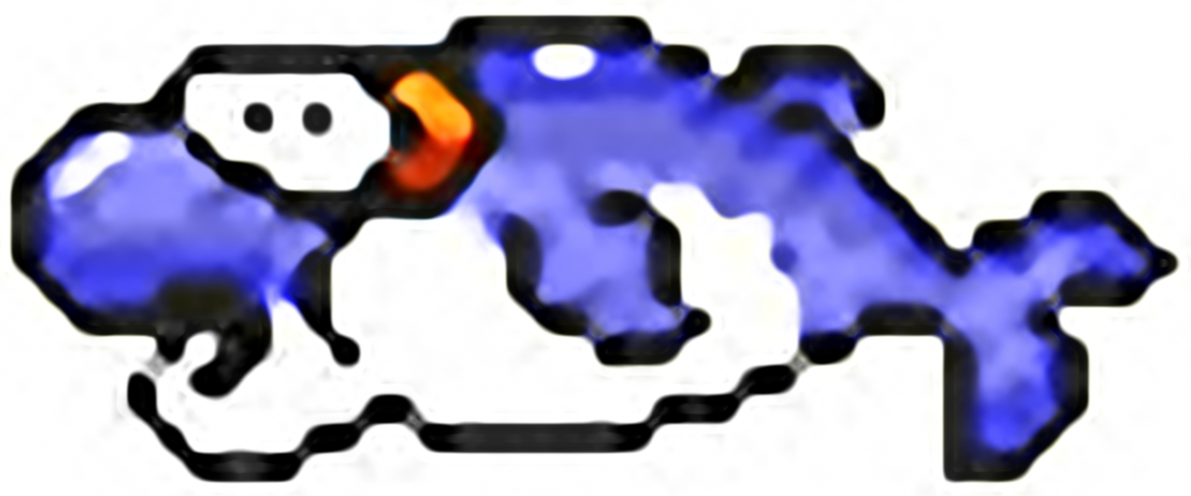
\includegraphics[width=0.45\textwidth]{img/dolphin_photozoom.png}
		\label{fig:zoom}
	}
	\subfigure[hq4x (Specialized Pixel Art Upscaling)]{
		
\includegraphics[width=0.45\textwidth]{img/dolphin_hq4x.png}
  		\label{fig:hq}
	}
	\subfigure[Adobe Live Trace (Vectorization)]{
		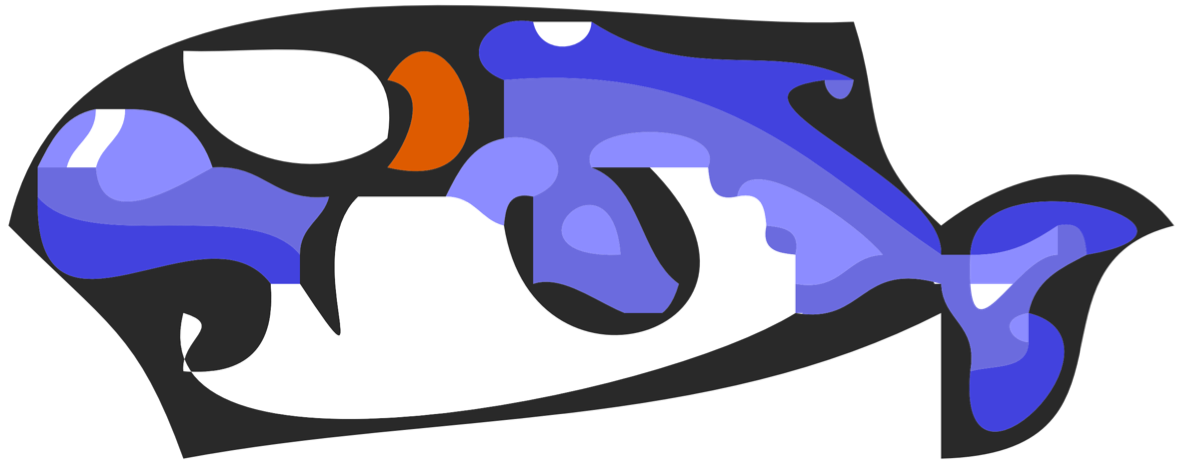
\includegraphics[width=0.45\textwidth]{img/dolphin_livetrace.png}
  		\label{fig:livetrace}
	}
	\caption{Results achieved with representatives of different categories of algorithms. (Input image \copyright Nintendo Co., Ltd.)}
\end{figure}


%%%%%%%%%%%

\subsection{General Image Upsampling} \label{sec:imageup}

Image interpolation works in two directions, and tries to achieve a best approximation of a pixel's color and intensity based on the values at surrounding pixels. Figure \ref{fig:interpol} illustrates how resizing/enlargement works.

\begin{figure} [ht]
	\centering
	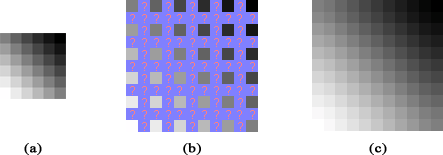
\includegraphics[scale=0.6]{img/interpolation.png}
	\caption{(a) Original image, magnified 2$\times$ (b) before interpolation (showing the unknown pixels) and (c) after interpolation.}
	\label{fig:interpol}
\end{figure}

\noindent The ``classical'' approach to image upsampling is to apply linear filters derived either from analytical interpolation or from signal processing theory. The most widely used methods are nearest-neighbor, bilinear, and bicubic interpolation (see Figure \ref{fig:nn-bl-bc3d}). Filters like these work by interpolating pixel color values, introducing a continuous transition into the output even where the original material has discrete transitions. They make no assumptions about the underlying data, other than that it is essentially band-limited. Although this is desirable for continuous-tone images, some algorithms reduce contrast (sharp edges) in a way that may be undesirable for line art. As a consequence, images upsampled in this manner typically suffer from blurring of sharp edges and ringing (edge halo) artifacts.

\begin{figure}[ht]
	\centering
	\subfigure[]{
		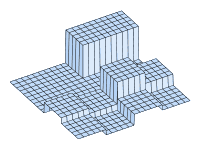
\includegraphics[width=0.3\textwidth]{img/3d_nearest.png}
		\label{fig:nn3d}
	}
	\subfigure[]{
		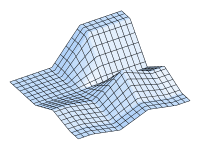
\includegraphics[width=0.3\textwidth]{img/3d_bilinear.png}
		\label{fig:bl3d}
	}
	\subfigure[]{
		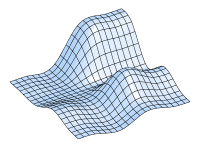
\includegraphics[width=0.3\textwidth]{img/3d_bicubic.png}
  		\label{fig:bc3d}
	}
	\caption{\subref{fig:nn3d} Nearest-neighbor, \subref{fig:bl3d} bilinear, and \subref{fig:bc3d} bicubic interpolation applied to the same uniformly-spaced input data.}
	\label{fig:nn-bl-bc3d}
\end{figure}

\noindent Common interpolation algorithms can be grouped into two categories: adaptive and non-adaptive. Adaptive methods change depending on what they are interpolating (sharp edges vs. smooth texture), whereas non-adaptive methods treat all pixels equally.
\begin{itemize}
	\item {\bf Non-adaptive algorithms} include: nearest-neighbor, bilinear, bicubic, spline, sinc, Lanczos \cite{Wolberg1990} and others. Depending on their complexity, these use anywhere from 0 to 256 (or more) adjacent pixels when interpolating. The more adjacent pixels they include, the more accurate they can become, but this comes at the expense of much longer processing time. These algorithms can be used to both distort and resize a photo.
	\item {\bf Adaptive algorithms} include many proprietary algorithms in licensed software such as: Qimage \cite{Qimage2012}, PhotoZoom Pro 4 \cite{Benvista2012}, Perfect Resize 7 \cite{Perfect2012}, SmartEdge \cite{Smartedge2007} and others. Many of these apply a different version of their algorithm (on a pixel-by-pixel basis) when they detect the presence of an edge -- aiming to minimize unsightly interpolation artifacts in regions where they are most apparent. These algorithms are primarily designed to maximize artifact-free detail in enlarged photos, so some cannot be used to distort or rotate an image.
\end{itemize}

\subsubsection{Non-adaptive methods}

Linear (non-adaptive) resampling methods are always a tradeoff between three artifacts: blur, aliasing, and ringing.\\\\
\begin{tabular}{m{0.8\textwidth} m{0.2\textwidth}}
	\begin{itemize}
		\item {\bf Blur} is a loss of image sharpness. It can be seen on images up-scaled using bilinear or bicubic interpolation.
	\end{itemize}
	&
	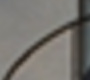
\includegraphics[scale=0.75]{img/blur.jpeg}
	\\
	\begin{itemize}
		\item {\bf Aliasing} appears as jagged edges (during up-scaling) or moire patterns (during down-scaling). It is present in images up-scaled using all linear methods, but it is most visible with nearest-neighbor, bicubic, and bilinear methods.
	\end{itemize}
	&
	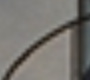
\includegraphics[scale=0.75]{img/aliasing.jpeg}
	\\
	\begin{itemize}
		\item {\bf Ringing} (also known as Gibbs phenomenon) appears as halo around edges. It is clearly visible with sinc, Lanczos, and bicubic methods. Some small amount of ringing improves the perceived sharpness of the image, but a high amount becomes annoying.
	\end{itemize}
	&
	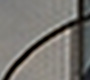
\includegraphics[scale=0.75]{img/ringing.jpeg}
\end{tabular}\\\\
It's important to understand that it's theoretically impossible to eliminate all of these artifacts simultaneously with linear methods.\\

{\bf Nearest-neighbor interpolation} is the most basic and requires the least processing time of all the interpolation algorithms because it only considers one pixel -- the closest one to the interpolated point. This algorithm selects the value of the nearest point and does not consider the values of neighboring points at all, yielding a piecewise-constant interpolant. This has the effect of simply making each pixel bigger and preserving all the original detail, but has undesirable jaggedness.\\

{\bf Bilinear interpolation} can be used where perfect image transformation with pixel matching is impossible, so that one can calculate and assign appropriate intensity values to pixels. Unlike other interpolation techniques such as nearest-neighbor interpolation and bicubic interpolation, bilinear interpolation considers only the closest 2$\times$2 neighborhood of known pixel values surrounding the unknown pixel's computed location. It then takes a weighted average of these 4 pixels to arrive at its final, interpolated value. The weight on each of the 4 pixel values is based on the computed pixel's distance (in 2D space) from each of the known points. This results in much smoother looking images than nearest-neighbor \cite{website:interpolation}.\\

{\bf Bicubic interpolation} goes one step beyond bilinear by considering the closest 4$\times$4 neighborhood of known pixels -- for a total of 16 pixels. Since these are at various distances from the unknown pixel, closer pixels are given a higher weighting in the calculation. Bicubic produces noticeably sharper images than the previous two methods, and is perhaps the ideal combination of processing time and output quality. For this reason it is a standard in many image editing programs (including Adobe Photoshop), printer drivers and in-camera interpolation \cite{website:interpolation}.\\

{\bf Higher order interpolation} take more surrounding pixels into consideration, and are thus also much more computationally intensive. These algorithms include {\bf spline and sinc}, and retain the most image information after an interpolation. They are therefore extremely useful when the image requires multiple rotations/distortions in separate steps. However, for single-step enlargements or rotations, these higher-order algorithms provide diminishing visual improvement as processing time is increased \cite{website:interpolation}.\\

{\bf Spline interpolation} is a form of interpolation where the interpolant is a special type of piecewise polynomial called a spline, which is preferred over polynomial interpolation because the interpolation error can be made small even when using low degree polynomials for the spline. Spline interpolation also avoids the problem of Runge's phenomenon \cite{Runge1901} which occurs when interpolating between equidistant points with high degree polynomials.\\

{\bf Sinc interpolation} has the disadvantage of producing significant ripple artifacts (Gibbs phenomenon, also called \emph{ringing}) in aliased images at the vicinity of image edges (see Figure \ref{fig:sincedge}). This is because $sinc(x):=sin(\pi t)/(\pi t)$ decays slowly, at a rate of $1/x$, so the damage from meeting an edge is spread throughout the image \cite{Getreuer2011}.\\

{\bf The Lanczos filter} is a windowed form of the sinc filter. The sinc function is infinite in extent and produces ringing artifacts, and thus not directly usable in practice. Instead, one uses approximations, called windowed forms of the filter and the Lanczos filter is one such windowing. The windows vanish outside of a range, and using larger ranges allows one to improve accuracy in exchange for more computation. Some have compared the Lanczos filter favorably with simpler filters or other windowings of sinc, finding it the ``best compromise'' among filters considered \cite{Turkowski1990}.

\begin{figure}[ht]
	\centering
	\subfigure[Nearest-neighbor]{
		
\includegraphics[width=0.15\textwidth]{img/edge_nn.png}
		\label{fig:nnedge}
	}
	\subfigure[Bilinear]{
		
\includegraphics[width=0.15\textwidth]{img/edge_bl.png}
		\label{fig:bledge}
	}
	\subfigure[Bicubic]{
		
\includegraphics[width=0.15\textwidth]{img/edge_bc.png}
  		\label{fig:bcedge}
	}
	\subfigure[Spline]{
		
\includegraphics[width=0.15\textwidth]{img/edge_spline.png}
  		\label{fig:splineedge}
	}
	\subfigure[Sinc]{
		
\includegraphics[width=0.15\textwidth]{img/edge_sinc.png}
  		\label{fig:sincedge}
	}
	\subfigure[Lanczos]{
		
\includegraphics[width=0.15\textwidth]{img/edge_lanczos.png}
  		\label{fig:lanczosedge}
	}
	\caption{Linear interpolation of a step edge. All non-adaptive interpolators attempt to find an optimal balance between three undesirable artifacts: aliasing, blurring and ringing.}
	\label{fig:nonadaptive}
\end{figure}

\noindent Even the most basic non-adaptive methods do quite well at preserving smooth tonal gradations, but they all begin to show their limitations when they try to interpolate near a sharp edge. Nevertheless, also the most advanced non-adaptive interpolators always have to increase or decrease one of the three artifacts at the expense of the others -- therefore at least one will be visible.

\subsubsection{Adaptive methods}

Adaptive (edge-detecting) algorithms do not treat all pixels equally, but instead adapt depending on nearby image content. This flexibility gives much sharper images with fewer artifacts (than would be possible with a non-adaptive method). Unfortunately, these often require more processing time, are usually more expensive and produce different kind of artifacts.\\
\begin{tabular}{m{0.65\textwidth} m{2.2cm} m{2cm}}
	\begin{itemize}
		\item {\bf Random pixels} appear sometimes in or near smooth image areas.
	\end{itemize}
	&
	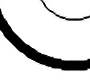
\includegraphics[scale=0.8]{img/random1.jpeg}
	&
	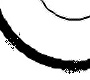
\includegraphics[scale=0.8]{img/random2.jpeg}
	\\
	\begin{itemize}
		\item {\bf Pattern areas} can have large artifacts. They become visible in areas of repeating patterns of small size.
	\end{itemize}
	&
	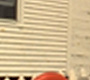
\includegraphics[scale=0.8]{img/pattern1.jpeg}
	&
	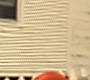
\includegraphics[scale=0.8]{img/pattern2.jpeg}
	\\
	\begin{itemize}
		\item {\bf Areas of fine structure} can look unnatural. This includes many natural textures, such as leaves, grass, clouds, water.
	\end{itemize}
	&
	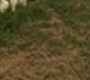
\includegraphics[scale=0.8]{img/grass1.jpeg}
	&
	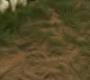
\includegraphics[scale=0.8]{img/grass2.jpeg}
\end{tabular}\\\\


{\bf Perfect Resize 7} (previously known as Genuine Fractals) is perhaps the most common iterative (or fractal) enlargement software. It tries to encode a photo similar to a vector graphics file -- allowing for near lossless resizing ability (at least in theory). Interestingly, its original aim was not for enlargement at all, but was instead intended for efficient image compression. Times have changed since storage space is now more plentiful and fortunately, so has its application \cite{Perfect2012}.\\

{\bf PhotoZoom Pro 4} (formerly S-Spline Pro) is another common enlargement program. It takes into account many surrounding pixels when interpolating each pixel, and attempts to re-create a smooth edge that passes through all known pixels. It uses a spline algorithm to re-create these edges, which is similarly used by car manufacturers when they design a new smooth-flowing body for their cars. PhotoZoom has several settings -- each geared towards a different type of image \cite{Benvista2012}.\\

{\bf SmartEdge} algorithm was developed by the Graphics and Media Lab of a State University of Moscow (MSU) in a joint research project with Samsung Electronics. SmartEdge 2 algorithm is a newer version of SmartEdge algorithm developed for top-notch quality upscaling \cite{Smartedge2007}.

\begin{figure}[ht]
	\centering
	\subfigure[Nearest-neighbor]{
		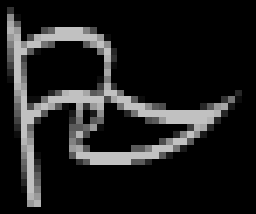
\includegraphics[width=0.2\textwidth]{img/enlarge_ex1_NN.png}
		\label{fig:nnlarge}
	}
	\subfigure[Perfect Resize 7]{
		
\includegraphics[width=0.2\textwidth]{img/enlarge_ex1_GF1.jpeg}
		\label{fig:prlarge}
	}
	\subfigure[PhotoZoom Pro 4]{
		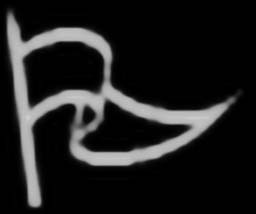
\includegraphics[width=0.2\textwidth]{img/enlarge_ex1_PZ1.jpeg}
  		\label{fig:pzlarge}
	}
	\subfigure[SmartEdge]{
		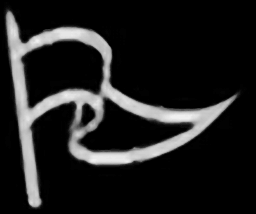
\includegraphics[width=0.2\textwidth]{img/enlarge_ex1_SE.png}
  		\label{fig:selarge}
	}
	\caption{Adaptive algorithms applied to a flag image.}
	\label{fig:adaptive}
\end{figure}

In the last decade, many other sophisticated algorithms have appeared which make stronger assumptions about the image, e.g. assuming natural image statistics \cite{Fattal2007} or self-similarity \cite{Glasner2009}. However, in most cases, these (natural) image assumptions do not hold for color-quantized, tiny pixel art images. For this reason, these methods tend to perform poorly on such inputs (see Figure \ref{fig:boofattal}).

\begin{figure}[ht]
	\centering
	\subfigure[]{
		
\includegraphics[width=0.2\textwidth]{img/smw_boo_nearest_9x.png}
		\label{fig:boonn}
	}
	\subfigure[]{
		
\includegraphics[width=0.2\textwidth]{img/smw_boo_freedman_9x.png}
		\label{fig:boofattal}
	}
	\caption{Example of an algorithm with natural image assumptions (Freedman and Fattal \cite{Fattal2007}) applied to pixel art (Boo \copyright Nintendo Co., Ltd.)}
\end{figure}

%%%%%%%%%%%

\subsection{Pixel Art Upscaling Techniques} \label{sec:pixelartup}

A number of specialized pixel art upscaling algorithms have been developed over the years \cite{Wiki:scaling}. Most of these have their origins in the emulation community. None has been published in a scientific venue; however, open source implementations are available for most. All of these algorithms are pixel-based and upscale the image by a fixed integer factor.\\

\begin{wrapfigure}[13]{r}{0.43\textwidth}
 	\centering
	\subfigure[Nearest-neighbor (16$\times$)]{
		
\includegraphics[width=0.20\textwidth]{img/invaders_01_nearest_16x.png}
		\label{fig:invnn}
	}
	\subfigure[EPX (16$\times$)]{
		
\includegraphics[width=0.20\textwidth]{img/invaders_01_epx_16x.png}
		\label{fig:invepx}
	}
	\caption{EPX limitations for ambiguous pixel connectivity. (Invaders \copyright Taito Corp.)}
	\label{fig:epx}
\end{wrapfigure}

\indent {\bf EPX (Eric's Pixel Expansion)} is the first algorithm of this type that we are aware of, and was developed by Eric Johnston in 1992 when porting the SCUMM engine games from the IBM PC (which ran at 320$\times$200$\times$256 colors) to the early color Macintosh computers, which ran at about double that resolution \cite{Kas1999}. The algorithm doubles the resolution of an image using a simple logic: every pixel is initially replaced by 2$\times$2 block of the same color; however, if the left and upper neighbors in the original image had the same color, that color would replace the top left pixel in the 2$\times$2 block, and analogously for the other corners. The algorithm is simple enough to be applied in real-time on emulators (see Figure \ref{fig:snes}) and often achieves good results. However, the direction of edges is quantized to only 12 distinct directions which can cause the results to appear blocky. Another limitation is in the strict local nature of the algorithm which prevents it from correctly resolving ambiguous connectivity of diagonal pixels (see Figure \ref{fig:invepx}).\\

{\bf Eagle} (by Dirk Stevens) \cite{website:eagle}, {\bf 2$\times$SaI} \cite{Liauw2001}, {\bf AdvMAME2$\times$} \cite{Wiki:scaling} and {\bf Scale2$\times$} \cite{Mazzoleni2001} are the best known algorithms based on the same idea of EPX, but use more sophisticated logic to determine the colors of the 2$\times$2 block, with larger causal neighborhoods and blending of colors. Several slightly different implementations exist under different names, such as {\bf SuperEagle} and {\bf Super2$\times$SaI}. An inherent limitation of all these algorithms is that they only allow upscaling by a factor of two. Larger magnification can be achieved by applying the algorithm multiple times, each time doubling the resolution (the AdvMAME4$\times$/Scale4$\times$ algorithm is just EPX applied twice to get 4$\times$ resolution). This strategy, however, significantly reduces quality at larger upscaling factors, because the methods assume non-antialiased input, while producing antialiased output.\\

The {\bf hq{\it n}x family} \cite{Stepin2003} is the latest and most sophisticated evolution of this type of algorithms. This algorithm examines 3$\times$3 pixel blocks at a time and compares the center pixel to its 8 neighbors. Each neighbor is classified as being either similar or dissimilar in color, which leads to 256 possible combinations. The algorithm uses a lookup table to apply a custom interpolation scheme for each combination. This enables it to produce various shapes, such as sharp corners, etc. The quality of the results is high. However, due to its strictly local nature, the algorithm cannot resolve certain ambiguous patterns and is still prone to produce staircasing artifacts. Lookup tables exist only for 2$\times$, 3$\times$, and 4$\times$ magnification factors, called hq2x, hq3x, and hq4x respectively.

\begin{figure}[ht]
	\centering
	\subfigure[Nearest-neighbor (16$\times$)]{
		
\includegraphics[width=0.183\textwidth]{img/smw_mushroom_nearest_16x.png}
		\label{fig:mushnn}
	}
	\subfigure[EPX (16$\times$)]{
		\includegraphics[width=0.183\textwidth]{img/smw_mushroom_epx_16x.png}
		\label{fig:mushepx}
	}
	\subfigure[SuperEagle (16$\times$)]{
		\includegraphics[width=0.183\textwidth]{img/smw_mushroom_supereagle_16x.png}
		\label{fig:mushse}
	}
	\subfigure[Super2$\times$SaI (16$\times$)]{
		\includegraphics[width=0.183\textwidth]{img/smw_mushroom_super2xsai_16x.png}
		\label{fig:mushssai}
	}
	\subfigure[hq4x (16$\times$)]{
		\includegraphics[width=0.183\textwidth]{img/smw_mushroom_hq4x_16x.png}
		\label{fig:mushhq4x}
	}
	\caption{Comparison of different pixel art upscaling algorithms. (Mushroom \copyright Nintendo Co., Ltd.)}
	\label{fig:upscaling}
\end{figure}

\begin{figure}[ht!]
	\centering
	\subfigure[Nearest-neighbor (2$\times$)]{
		\includegraphics[width=0.75\textwidth]{img/SNES_SMW_screen_nearest_neighbour_2x.png}
		\label{fig:snesnn}
	}
	\subfigure[EPX (2$\times$)]{
		\includegraphics[width=0.75\textwidth]{img/SNES_SMW_screen_scale2x.png}
		\label{fig:snesepxl}
	}
	\caption{Application of the EPX algorithm to a frame from ``Super Mario World'' of the \emph{Super Nintendo Entertainment System}. (Input image \copyright Nintendo Co., Ltd.)}
	\label{fig:snes}
\end{figure}

%%%%%%%%%%%

\subsection{Image Vectorization} \label{sec:imagevect}

Unlike the opposite process of rasterization, vectorization is not well defined, meaning there is not a single correct method. Many different algorithms exist, and each gives different results, as vector representations are more abstract than pixels.\\
A large body of work deals with the automatic extraction of vector representations from images. However, most are designed with larger natural images in mind and rely on segmentation or edge detection algorithms to cluster many pixels into larger regions, to which vector curves and region primitives are fit. These clustering tools do not perform well on pixel art images, because features are tiny, all edges are step edges, and there are no gradients that can be followed downhill. For these reasons, all algorithms examined in this section (excluding Kopf-Lischinski) tend to lose the small features characteristic to pixel art.\\
Another challenge for these algorithms is dealing with 8-connected pixels; many pixel art images contain thin features that are only connected through pixel corners. General image vectorization tools are not designed to handle this situation and the ambiguities that arise from it and consequently tend to break the connectivity of these features.\\

The first vectorization systems were designed to convert black-and-white images consisting primarily of thin lines into vector images in which the basic shapes are line segments. This type of image, commonly called a ``line drawing'', is frequently used for figures in engineering, science, mathematics, or other fields. Line drawings may contain curves in addition to lines. \\
Examples of such vectorization systems include early research by Freeman \cite{Freeman1961} and some later work by Chiang \cite{Chiang1995}, Dori and Liu \cite{Dori1999}, and Jennings and Parker \cite{Jennings1994}. Song et al. describe two different line drawing vectorization schemes in 2000 and 2002 \cite{Song2000, Song2002}. These systems primarily focus on vectorizing engineering drawings. Boatto et al. created a system for vectorizing maps that makes use of line drawing vectorization schemes \cite{Boatto1992}. Tanaka, Kamimura, and Shashkov present another map vectorization scheme that focuses mainly on the line drawing portions of the map \cite{Tanaka1993}]. Selinger describes an algorithm dubbed Potrace for tracing binary images and presents results on very tiny images \cite{Selinger2003} (see Figure \ref{fig:wheelpot}).

\begin{figure}[ht]
	\centering
	\subfigure[Nearest-neighbor]{
		\includegraphics[width=0.4\textwidth]{img/wheel.png}
		\label{fig:wheelnn}
	}
	\subfigure[Potrace]{
		\includegraphics[width=0.4\textwidth]{img/wheel.eps}
		\label{fig:wheelpot}
	}
	\caption{Black-and-white image vectorized using Potrace.}
	\label{fig:potrace}
\end{figure}

The process of converting a line drawing from raster to vector form is called vectorization because the line segments produced by early systems are represented as vectors relative to the endpoint of the previous line. Since that time, the terms vectorization and vector image have become more general to include other types of images.\\
This type of vectorization consists of fitting a line to groups of neighboring black pixels that are in a straight line. Because of the discrete nature of the raster image, the pixels form a straight line only in very unusual circumstances. Normally, they are simply almost in a straight line, and some method must approximate the line from the pixel locations. Additionally, it can be difficult to determine whether the variations from one pixel to the next are because of the discrete nature of the line, or because the pixels belong to different lines.\\
It is possible to represent a curve as a series of short, connected line segments, but a smoother result is achieved by including curves in the vectorization. While curves are more difficult to vectorize than lines, the approach is still the same: identify pixels that belong together, and fit a curve to them. Enforcing continuity between curves is also challenging. It can be difficult to determine the degree of continuity at a transition, and it can be difficult to pick curves that are continuous to the desired degree and approximate the pixels accurately.\\
The type of curve used varies from one vectorization system to the next; many systems use circular arcs, conic sections, B\'ezier curves, or B-splines to represent curves. Hori and Tanigawa \cite{Hori1993}, and R\"o\"osli and Monagan \cite{Roosli1995} use straight line segments and circular arcs. Nagasamy and Lagrana approximate curves using conic sections \cite{Nagasamy1990}. Chang and Yan use B\'ezier curves to approximate the drawing \cite{Chang1998}. Kopf and Lischinski use cubic B-splines to approximate the nodes of reshaped pixel cells \cite{Kopf2011}.\\
There are several factors to consider when choosing the representation of curves in the vector image. In order to allow the greatest flexibility, the curves should be able to represent many kinds of objects. For this reason, circular arcs are not a good choice.\\
One should also choose curves that are easy to edit. Most shapes are defined using a set of control points. The control points should at least lie near the curve, and it is better for the control points to lie on the curve. Moving the control points changes the shape, and the resulting change should be predictable. Generally, a curve is easier to edit if it has only a few control points, so a vector image should be defined with as few control points as possible.\\
B-spline curves and surfaces have many good properties for the basic shape in a vector image. For those unfamiliar with B-splines, there is a more detailed description in Section \ref{sec:bsplines}. B-splines are made of a set of control points that lie near the curve but generally do not lie on the curve (unless they are interpolated). B-splines are easy to edit because moving the control points changes the curve predictably, and moving a particular control point only changes the portion of the curve near that point. The mathematics of B-splines allow various degrees of continuity to produce smooth shapes or sharp corners.

If we introduce color (or gray scale) into a line image, we can still use the basic line image vectorization described above with minor modifications. These color images have to be quantized and decomposed into separate binary channels first, which are then traced separately (which can result in inter-penetrating shapes). First, the background color must be chosen. For a line drawing, this is normally the most common color in the image. The lines (or curves) can be identified as groups of pixels that are a different color than the background. This may be difficult if the image is noisy (there are small random variations in color). Once the pixels are identified, they are approximated with a line or curve, and a color is chosen to match the color of the pixels.\\
Black and white pictures often contain large regions that are all black, violating the definition of a line drawing. To vectorize such images, a region-based vectorization system is used. Such a system is similar to line-drawing vectorization, but approximates region boundaries with lines and curves.\\
Kasturi et al. describe a system for vectorizing line drawings that also allows the drawings to contain solid binary regions, whose outlines are approximated, so this vectorization scheme fits into both the region and line vectorization categories \cite{Kasturi1990}. Likewise, Nagasamy and Lagrana vectorize engineering drawings that may contain large solid objects by approximating the boundaries of the solid objects \cite{Nagasamy1990}. Jimenez and Navalon use a region-based vectorization scheme, but the result is a set of polygon boundaries, not smoother curves \cite{Jimenez1982}. Mikheev, Vincent, and Faber propose another system for vectorization based on region boundaries, but it is only designed to approximate polygons, not smooth curves \cite{Mikheev2001}. Yang, Lu, and Lee use B\'ezier curves to approximate the outlines of Chinese calligraphy characters \cite{Yang2001}.\\
A region-based vectorization system can also be extended to include color by requiring all pixels within a region to be the same color. First, the image is divided into sets of consecutive pixels that have the same color. Next, the boundary of each of those regions is approximated with appropriate curves. Finally, the shape is assigned a color based on the color of the pixels.\\
Although filling each shape with a single color is common, real objects are seldom filled with a single color. For example, a picture taken with a digital camera usually contains objects with varying color, so it is better to vectorize those objects using shapes that vary in color. It is harder to determine which regions belong together when they are not uniform in color. The gradient color of each region must be approximated instead of simply assigning a single color to the entire region.\\
Ge describes a system to approximate images using a set of triangles \cite{Ge2001}. Although the intended use of this triangulation system is image morphing, it could easily be seen as a region-based vectorization system. Its primary advantage over other vectorization systems is that it approximates gradient colors. However, it still has many shortcomings when used for vectorization. One is that both the region boundaries and the color are approximated using linear shapes, so the result is by no means smooth. This also means that in order to approximate curves and regions that are not linearly shaded, the algorithm produces an unnecessarily large number of control points (triangle vertices), making the image difficult to edit. The result is also not well suited for user editing because it fails to segment the image into objects, nor does it layer those objects. If the user wishes to move an object, it is necessary to group all the triangles that belong to the object and manually set the layer.\\
Armstrong describes an algorithm where the image is first segmented, and the segments are then layered \cite{Armstrong2006}. The boundary of each segment is approximated with a periodic B-spline curve, which is then used to create a B-spline surface to approximate the interior of the segment. The algorithm fits each B-spline to the colors of the image using least-squares approximation, with the color and shape of each B-spline surface being extrapolated into regions behind other segments. The result is a vector image made of layered B-spline surfaces. Figure \ref{fig:armstrong} gives an overview of the algorithm.

\begin{figure}[ht]
	\centering
	\subfigure[]{
		\includegraphics[height=3.5cm]{img/rose1.png}
		\label{fig:rose1}
	}
	\subfigure[]{
		\includegraphics[height=3.5cm]{img/rose2.png}
		\label{fig:rose2}
	}
	\subfigure[]{
		\includegraphics[height=3.5cm]{img/rose3.png}
		\label{fig:rose3}
	}
	\subfigure[]{
		\includegraphics[height=3.5cm]{img/rose4.png}
		\label{fig:rose4}
	}
	\subfigure[]{
		\includegraphics[height=3.5cm]{img/rose5.png}
		\label{fig:rose5}
	}
	\caption{Overview of the algorithm described by Armstrong: the original image \subref{fig:rose1} is first segmented and layered \subref{fig:rose2}, the boundary of the segments are then approximated \subref{fig:rose3} and converted into B-spline surfaces \subref{fig:rose4}, and the colors approximated with gradients \subref{fig:rose5}.}
	\label{fig:armstrong}
\end{figure}

Another vectorization algorithm is being developed by Price \cite{Price2006}. It approximates regions with B\'ezier patches and then refines the approximation by subdividing the patches. This is repeated until the approximation is sufficient within a user-defined threshold.\\
Lecot and L\'evy present a system (``ARDECO''), an algorithm that computes a set of vector primitives and first- or second-order gradients that best approximates the image \cite{Lecot2006}. Lai et al. present an algorithm for automatic extraction of gradient meshes from raster images \cite{Lai2009}. Also this algorithms rely on segmentation, which are unlikely to work satisfactorily on pixel art images.\\
Orzan et al. introduce image partitioning diffusion curves, which diffuse different colors on both sides of the curve \cite{Orzan2008}. In their work, they also describe an algorithm for automatically extracting this representation from a raster image. Their formulation, however, relies on Canny edge detection. These filters do not work well on pixel art input, most likely due to the small image size, since edge detectors have a finite support. Xia et al. describe a technique that operates on a pixel level triangulation of the raster image \cite{Xia2009}. However, it also relies on Canny edge detection.\\

There are currently many commercial vectorization products. For example, the Adobe Image Trace program (previously known as Streamline and then as Live Trace) \cite{Adobe2012} and Vector Magic \cite{Vector2010} convert drawings into a vector format based on B\'ezier curves. In general, these commercial products are geared toward vectorizing line drawings, regions of similar color, or text. Their documentation usually suggests not to use them on actual photographs because of the difficulty in vectorizing photographs. The exact nature of the underlying algorithms is not disclosed, however, they generally do not perform well on pixel art images (see Figures \ref{fig:livetrace} and \ref{fig:livetracemush}).

\begin{figure}[ht]
	\centering
	\subfigure[Nearest-neighbor (16$\times$)]{
		\includegraphics[height=4cm]{img/smw_mushroom_nearest_16x.png}
		\label{fig:nnmush}
	}
	\subfigure[Adobe Image Trace (16$\times$)]{
		\includegraphics[height=4cm]{img/smw_mushroom_livetrace_16x.png}
		\label{fig:livetracemush}
	}
	\caption{Vectorization technique applied to pixel art (compare to pixel art upscaling techniques in Figure \ref{fig:upscaling}).  (Mushroom \copyright Nintendo Co., Ltd.)}
	\label{fig:smw_mush}
\end{figure}

The Kopf-Lischinski algorithm is a novel way to extract resolution-independent vectors from pixel art described in the 2011 paper ``Depixelizing Pixel Art'' \cite{Kopf2011}. This project is based on the Kopf-Lischinski algorithm, whose steps and procedure are explained in Section \ref{sec:design}.

%%%%%%%%%%%%%%%%%%%%%%%%%
\section{Project requirements and analysis}
%%%%%%%%%%%%%%%%%%%%%%%%%

\subsection{Challenges}
The goal in this work is to convert pixel art images to a resolution-independent vector representation, where regions with smoothly varying shadings are crisply separated by piecewise-smooth contour curves. While this is also the goal of general image vectorization algorithms, the unique nature of pixel art images poses some non-trivial challenges:
\begin{itemize}
	\item \emph{Every pixel matters}. For example, a single pixel whose color is sufficiently different from its surrounding neighborhood is typically a feature that must be preserved (e.g., a character's eye).
	\item \emph{Pixel-wide 8-connected lines and curves} are features that appear visually connected at the original small scale, but become visually disconnected under magnification.
	\item \emph{Locally ambiguous configurations}: for example, when considering a 2$\times$2 checkerboard pattern with two different colors, it is unclear which of the two diagonals should be connected as part of a continuous feature line. This problem has been studied in the context of foreground/background separation in binary images, and simple solutions have been proposed \cite{Kong1996}. The challenge, however, is more intricate in the presence of multiple colors.
	\item The jaggies in pixel art are of a large scale compared to the size of the image, making it \emph{difficult to distinguish between features and pixelization artifacts}.
\end{itemize}

%%%%%%%%%%%

\subsection{Algorithm overview}
The main primitive in the vector representation described by Kopf and Lischinski are quadratic B-spline curves \cite{Kopf2011}, that in my implementation are later converted into sequences of B\'ezier curves (see why in Section \ref{sec:extractbezier}). This curves define the piecewise smooth contours between regions. Thus, the main computational task is to determine the location and the precise geometry of these contours. Similarly to other vectorization algorithms, this boils down to detecting the edges in the input pixel art image and fitting curves of the proper shape to them. However, this process is complicated by the reasons listed above.\\
Because of the small scale of pixel art images and the use of a limited color palette, localizing the edges is typically easy: any two adjacent pixels with sufficiently different colors should be separated by a contour in the vectorized result. However, the challenge lies in connecting these edge segments together, while correctly handling 8-connected pixels and resolving local ambiguities.\\
Consider a square lattice graph with $(w+1)\times(h+1)$ nodes, representing a $w\times h$ image. Each pixel corresponds to a closed cell in this graph. Horizontal and vertical neighbor cells share an edge in this graph, while diagonal neighbors share only a vertex. These diagonal neighbors become visually disconnected when the lattice is magnified, while the neighbors that share an edge remain visually connected. Thus, the first step in the Kopf-Lischinski algorithm \cite{Kopf2011} is to reshape the original square pixel cells so that every pair of neighboring pixels along a thin feature, which should remain connected in the vectorized result, correspond to cells that share an edge. In this process, described in Section \ref{sec:ambiguities}, a few carefully designed heuristics are employed to resolve locally ambiguous diagonal configurations.\\
Having reshaped the graph, we identify edges where the meeting pixels are part of different components (the main shapes of the vector representation). We refer to these edges as visible because they form the basis for the visible contours of the components in the final vector representation, whereas the remaining edges will not be visible as they are ignored in the successive steps. \\
To produce smooth contours, quadratic B-spline curves are fitted to sequences of visible edges (contours), as described in Section \ref{sec:fitsplines}. However, because the locations of the curve control points are highly quantized due to the low-resolution underlying pixel grid, the results might still exhibit staircasing. The curve shapes are therefore smoothed to reduce the staircasing effects, while preserving intentional high-curvature features (corners) along each contour, as described in Section \ref{sec:smooth}.\\
The image is then finalized by adding the colors of each component and using radial gradients for the shadings (see Section \ref{sec:shadings}), and is saved as a SVG file.\\\\
The following is a summary of the main steps in the algorithm (see also Figure \ref{fig:algo}), each described in detail in Section \ref{sec:design}:
\begin{enumerate}
	\item get as input a raster image in any of the following formats: bmp, jpg, gif, png;
	\item resolve all separation/connectedness ambiguities of the original pixel grid;
	\item reshape the pixel cells, such that connected neighboring pixels (whether in cardinal or diagonal direction) share an edge;
	\item find, merge and segment visually significant edges (contours); 
	\item build the components shapes;
	\item fit spline curves to visually significant edges;
	\item optimize spline curves' control points to maximize smoothness and reduce stair-casing artifacts;
	\item introduce diffusion solvers where there are regions with smoothly varying shading;
	\item return a vector representation (SVG file) that can be rendered at any resolution.
\end{enumerate}

\begin{figure}[ht]
	\centering
	\subfigure[]{
		\includegraphics[width=0.42\textwidth]{img/detail_anti_venom1.png}
		\label{fig:av1}
	}
	\subfigure[]{
		\includegraphics[width=0.42\textwidth]{img/detail_anti_venom2.png}
		\label{fig:av2}
	}
	\subfigure[]{
		\includegraphics[width=0.42\textwidth]{img/detail_anti_venom3.png}
		\label{fig:av3}
	}
	\subfigure[]{
		\includegraphics[width=0.42\textwidth]{img/detail_anti_venom4.png}
		\label{fig:av4}
	}
	\subfigure[]{
		\includegraphics[width=0.42\textwidth]{img/detail_anti_venom6.png}
		\label{fig:av6}
	}
	\subfigure[]{
		\includegraphics[width=0.42\textwidth]{img/detail_anti_venom7.png}
		\label{fig:av7}
	}
	\caption{Overview of the algorithm. \subref{fig:av1} Detail of the input image. \subref{fig:av2} Initial similarity graph with crossing edges highlighted by red circles. The edges that lie inside flat shaded regions have been removed and the crossing edges solved. \subref{fig:av3} Reshaped pixel cells reflecting the connections in the resolved similarity graph. \subref{fig:av4} Computed contours (visible edges). \subref{fig:av6} Splines fit to visible edges. \subref{fig:av7} Final result with smoothed splines to reduce staircasing artifacts and shadings (top right).}
	\label{fig:algo}
\end{figure}

%%%%%%%%%%%

\subsection{Programming language}

The first choice I had to make in this project was the programming language used to implement the algorithm. Because of my experience and knowledge, this choice was mainly restricted to three programming language: Java, C and C++. \\
Since the resulting application has to manage images and graphic components, I discarded C almost immediately because of the complexity in performing even the simplest task, like extracting pixel values from raster images. Being C such a low level programming language means that many features and functions have to implemented from scratch, while in other languages this are already a default. \\
Although C++ might have a great potential, I'm not too confident about its features and libraries, and my knowledge of this programming language is not very thorough.\\
This lead me to Java, a programming language that I've already used in other projects before and I'm pretty confident working with. I've had some experiences with Java's graphic user interfaces (Swing and AWT) and I discovered that reading pixel's values from a raster image is extremely simple and format independent (any raster image in the formats bmp, jpg, gif and png can be used) (see Section \ref{sec:similarity}). Furthermore, after some research on libraries for vector graphics, I found a pure-Java library to render, generate, and manipulate SVG graphics: the Apache Batik library \cite{Batik} (see Section \ref{sec:result} for further details). This discovery finalized my choice.

%%%%%%%%%%%

\subsection{Vector file format} \label{sec:formats}

The application implemented in this project computes a vector representation at the end of the whole process. This representation has to be formatted to comply with a chosen standard, since one of the requirements states that a vector file has to be returned.\\
There are different vector file format available nowadays, common ones include:
\begin{itemize}
	\item EPS (Encapsulated PostScript): a DSC-conforming PostScript document with additional restrictions which is intended to be usable as a graphics file format.
	\item AI and CDR: vector files created by two most popular vector graphics programs, Adobe Illustrator and CorelDRAW respectively.
	\item WMF/EMF (Windows MetaFile/Enhanced MetaFile): Microsoft-created graphics file format containing both bitmaps and vectors. 
	\item SVG (Scalable Vector Graphics): a vector file format created with the Internet in mind and supported by Internet browsers.
\end{itemize}

\begin{wrapfigure}[23]{r}{0.27\textwidth}
 	\centering
	\vspace{-0.5cm}
	\includegraphics[width=0.25\textwidth]{img/phone.png}
  	\caption{A cordless phone. An example of how artists can achieve photo realistic results using the SVG format.}
	\label{fig:phone}
\end{wrapfigure}

\noindent After considering the most popular vector formats, I chose the Scalable Vector Graphics (SVG) standard as the preferable to use in the project.\\
Scalable Vector Graphics (SVG) is a family of specifications of an XML-based file format for two-dimensional vector graphics, both static and dynamic (i.e., interactive or animated). The SVG specification is an open standard that has been under development by the World Wide Web Consortium (W3C) since 1999 \cite{Wiki:formats}.\\
SVG images and their behaviors are defined in XML text files. This means that they can be searched, indexed, scripted, and, if need be, compressed. As XML files, SVG images can be created and edited with any text editor, but it is often more convenient to create them with drawing programs such as Inkscape. Because of my previous experiences with HTML and DOM, being SVG a XML-based file format has been a further advantage over other vector formats.\\
All major modern web browsers have at least some degree of support for SVG and can render markup directly, including Mozilla Firefox, Internet Explorer 9, Google Chrome, Opera, and Safari. Earlier versions of Microsoft Internet Explorer (IE) do not support SVG natively \cite{Wiki:svg}.\\
In recent years, Scalable Vector Graphics (SVG) has become a significant format that is completely independent of the resolution of the rendering device, typically a printer or display monitor. SVG files are essentially printable text that describes both straight and curved paths, as well as other attributes. Rendering SVG requires conversion to raster format at a resolution appropriate for the current task. SVG is also a format for animated graphics \cite{Wiki:vector}.\\
SVG allows three types of graphic objects: vector graphics, raster graphics, and text. Graphical objects, including PNG and JPEG raster images, can be grouped, styled, transformed, and composited into previously rendered objects. SVG does not directly support z-indices that separate drawing order from document order for overlapping objects, unlike some other vector markup languages like VML. Text can be in any XML namespace suitable to the application, which enhances search ability and accessibility of the SVG graphics. The feature set includes nested transformations, clipping paths, alpha masks, filter effects, template objects, and extensibility (see list below).\\
After choosing the programming language (Java) and finding the Batik library to manage SVG files, this format was definitely the best choice. I researched the potential and functions that the format offers, and the quality of the results that can be achieved is astonishingly high (see Figure \ref{fig:phone}).\\\\
The SVG 1.1 specification defines 14 functional areas or feature sets:
\begin{itemize}
	\item {\bf Paths}: simple or compound shape outlines are drawn with curved (B\'ezier and elliptical curves) or straight lines that can be filled in, outlined, or used as a clipping path.
	 \item {\bf Basic shapes}: straight-line paths and paths made up of a series of connected straight-line segments (polylines), as well as closed polygons, circles and ellipses can be drawn. Rectangles and round-cornered rectangles are also standard elements.
	\item {\bf Text}: unicode character text included in an SVG file is expressed as XML character data. Many visual effects are possible, and the SVG specification automatically handles bidirectional text, vertical text and characters along a curved path.
	\item {\bf Painting}: SVG shapes can be filled and/or outlined (painted with a color, a gradient, or a pattern). Fills can be opaque or have any degree of transparency. ``Markers'' are line-end features, such as arrowheads, or symbols that can appear at the vertices of a polygon.
	\item {\bf Color}: colors can be applied to all visible SVG elements, either directly or via `fill', `stroke,' and other properties.
	\item {\bf Gradients and patterns}: SVG shapes can be filled or outlined with solid colors as above, or with color gradients or with repeating patterns. Color gradients can be linear or radial (circular), and can involve any number of colors as well as repeats. Opacity gradients can also be specified. Patterns are based on predefined raster or vector graphic objects, which can be repeated in x and/or y directions. Gradients and patterns can be animated and scripted.
	\item {\bf Clipping, masking and compositing}: graphic elements, including text, paths, basic shapes and combinations of these, can be used as outlines to define both 'inside' and 'outside' regions that can be painted (with colors, gradients and patterns) independently.
	\item {\bf Filter effects}: a filter effect consists of a series of graphics operations that are applied to a given source vector graphic to produce a modified bitmapped result.
	\item {\bf Interactivity}: SVG images can interact with users in many ways. In addition to hyperlinks as mentioned below, any part of an SVG image can be made receptive to user interface events such as changes in focus, mouse clicks, scrolling or zooming the image and other pointer, keyboard and document events.
	\item {\bf Linking}: SVG images can contain hyperlinks to other documents, using XLink. URLs of SVG images can specify geometrical transforms in the fragment section.
	\item {\bf Scripting}: all aspects of an SVG document can be accessed and manipulated using scripts in a similar way to HTML. 
	\item {\bf Animation}: SVG content can be animated using built-in animation elements. Animations can be continuous, they can loop and repeat, and they can respond to user events.
	\item {\bf Fonts}: as with HTML and CSS, text in SVG may reference external font files, such as system fonts.
	\item {\bf Metadata}: in accord with the W3C's Semantic Web initiative, SVG allows authors to provide metadata about SVG content.
\end{itemize}

\subsubsection{Planification}

At the beginning of the project I planned the workflow and the main steps of the implementation process. They follow very tightly the steps of the algorithm, translating the process into the effective evolution of the application.\\

\noindent The project can be divided in the following milestones, which represent end-points of process activities:
\begin{description}
	\item[Milestone 1:]~\\
	kick off meeting to explain the project rules and directives, and plan the development process.
	\item[Milestone 2:]~\\
	first prototype of the program that is able to process a raster image (analyze the pixel grid) and return a basic vector image. Implementation of an initial and basic interface.
	\item[Milestone 3:]~ \\
	basic algorithm that resolves all separation/connectedness ambiguities of the original pixel grid and reshapes the pixel cells.
	\item[Milestone 4:]~ \\
	implementation of the algorithm with fitting of spline curves to visible edges.
	\item[Milestone 5:]~ \\
	improve the smoothness of the curves by optimizing the locations of their control points. Also detect corners to avoid excessive approximation of the figure.
	\item[Milestone 6:]~ \\
	complete thesis, poster and final presentation of the project.
\end{description}

\begin{figure}[!ht]
	\centering
	\includegraphics[width=1\textwidth]{img/gantt_plan.png}
	\caption{Project tasks and milestones.}
\end{figure}

\newpage

%%%%%%%%%%%%%%%%%%%%%%%%%
\section{Project design} \label{sec:design}
%%%%%%%%%%%%%%%%%%%%%%%%%

\subsection{Raster to similarity graph} \label{sec:similarity}

The first step in the algorithm is to convert a raster image into a similarity graph, but we need first to extract the values of all pixels in the image. \\
In Java, the class {\tt ImageIO} has the method {\tt read(\emph{File})} which returns a {\tt BufferedImage} for files in the formats bmp, jpg, gif and png. This {\tt BufferedImage} class can be used to extract all color values from the image with the {\tt getRGB()} method. The values are then saved into a row-first ordered array and can be used to convert the bitmap into a similarity graph. \\
The similarity graph is a representation of the image, with the following characteristics:
\begin{itemize}
	\item each node corresponds to a pixel;
	\item edges represent connections between pixels that are part of the same component;
	\item red circles show where edges from different components intersect (ambiguities).
\end{itemize}
After a fully disconnected graph has been generated from the array of pixels, the connections are added by constructing the components.

\subsubsection{Construction of the components} \label{sec:constructcomp}

\begin{wrapfigure}[11]{r}{0.27\textwidth}
 	\centering
	\vspace{-1.cm}
	\includegraphics[width=0.25\textwidth]{img/moore.jpeg}
  	\caption{Moore neighborhood. Grey cells are in Moore neighborhood of red cell.}
	\label{fig:moore}
\end{wrapfigure}

Components are the fundamental object in the implementation, and they represent the vector objects in the final result. In the similarity graph, components are fully connected sub-graphs. They are constructed by starting from a chosen pixel and traversing the graph iteratively (not recursively, see Section \ref{sec:issuetraverse}) in all 8 directions. In this algorithm the type of connectivity between the pixels is 8-connected: pixels are neighbors to every pixel that touches one of their edges or corners. These pixels are connected horizontally, vertically, and diagonally (Moore neighborhood, see Figure \ref{fig:moore}).\\
The first pixel is added to a new component, and each pixel traversed afterwards is added to the same component. This iteration is repeated until all nodes have been traversed. Two conditions are available to guide the construction of the components, and can be selected or deselected at run-time:
\begin{itemize}
	\item {\bf merge similar colors} (to simplify the image): if enabled, pixels with similar colors are connected; if disabled, only pixels with the exact same color are connected (see Figure \ref{fig:merge}). Similarity is computed following the criteria used in the hqx algorithm \cite{Stepin2003}, where the YUV channels of the pixel and its neighbor are compared, considering them to be dissimilar if the difference in Y, U, V is larger than 48/255, 7/255, or 6/255 respectively. 
	\begin{figure}[ht]
		\centering
		\subfigure[Detail of the input image.]{
			\includegraphics[height=2.5cm]{img/merge1.png}
			\label{fig:merge1}
		}\\
		\subfigure[Similarity graph without merging.]{
			\includegraphics[height=3.5cm]{img/merge2.png}
			\label{fig:merge2}
		}
		\subfigure[Similarity graph with merging.]{
			\includegraphics[height=3.5cm]{img/merge3.png}
			\label{fig:merge3}
		}
		\caption{Merging similar colors simplifies the image, but the values of some pixels are overwritten.}
		\label{fig:merge}
	\end{figure}
	\item {\bf connect lines diagonally} (to smooth the contours): many pixel artists use different colors when drawing lines and contours of images, and can lead to some unexpected and unwanted artifacts since this lines are treated as disconnected (see Figure \ref{fig:connectlines5}). It is therefore possible to enable the option of merging this lines (components with only valence-2 nodes), which will connect them if their colors have a YUV distance of at most 100/255. Only diagonal connections are made, since horizontal and vertical discontinuities are not visible (see top right nodes of Figure \ref{fig:connectlines2}).
	\begin{figure}[ht]
		\centering
		\subfigure[Detail of the input image.]{
			\includegraphics[height=4.cm]{img/connect_lines1.png}
			\label{fig:connectlines1}
		}\\
		\subfigure[Similarity graph without connected lines.]{
			\includegraphics[height=5cm]{img/connect_lines4.png}
			\label{fig:connectlines4}
		}
		\subfigure[Similarity graph with connected lines.]{
			\includegraphics[height=5cm]{img/connect_lines2.png}
			\label{fig:connectlines2}
		}\\
		\subfigure[Final result without connected lines.]{
			\includegraphics[height=5cm]{img/connect_lines5.png}
			\label{fig:connectlines5}
		}
		\subfigure[Final result with connected lines.]{
			\includegraphics[height=5cm]{img/connect_lines3.png}
			\label{fig:connectlines3}
		}
		\caption{Connecting lines removes many staircasing artifacts, but removes the values of some pixels.}
		\label{fig:connectlines}
	\end{figure}
\end{itemize}
If one or both of this options is enabled, the components will contain pixels with different colors (see Figure \ref{fig:merge3}). In the final visualization only the major color is rendered (the color in most of the pixels), which can lead to a over-simplification of the image and a resulting loss in details. This can be partially prevented by enabling the shadings (see Section \ref{sec:shadings}), that add a radial gradient in the locations of the differently colored pixels (see Figure \ref{fig:connectlines3}).

\subsubsection{Finding the connectivity issues} \label{sec:findambig}

After the components have been constructed, some ambiguities can arise. If edges between different components intersect, they have to be solved. This are easily spotted: in the implementation each pixel is an object and contains its component's reference, so it's sufficient to check whether intersections happen between pixels with different component's references. If it's the case, the edges are marked as ambiguities with a red circle.

%%%%%%%%%%%

\subsection{Simplify graph and resolve ambiguities} \label{sec:ambiguities}

The graph processed in the previous step typically contains many crossing diagonal connections. The goal is now to eliminate all of these edge crossing in order to make the graph planar. The dual of the resulting planar graph will have the desired property of connected neighboring pixel cells sharing an edge, used to reshape the pixels in Section \ref{sec:reshape}.\\
We first distinguish between two cases:
\begin{enumerate}
	\item If a 2$\times$2 block is fully connected, all its nodes are part of the same component. In this case the two diagonal connections can be safely removed without affecting the final result. Such connections are visible in the green component of Figure \ref{fig:simplegraph1}.
	\item If a 2$\times$2 block only contains diagonal connections, and the nodes are not part of the same component, it means that removing one connection or the other will affect the final result. In this case we have to carefully choose which of the connections to remove. Such connections are highlighted by a red circle (see Figure \ref{fig:simplegraph}).
\end{enumerate}

\begin{figure}[ht]
		\centering
		\subfigure[Original similarity graph.]{
			\includegraphics[width=0.45\textwidth]{img/simple_graph1.png}
			\label{fig:simplegraph1}
		}
		\subfigure[Planar similarity graph.]{
			\includegraphics[width=0.45\textwidth]{img/simple_graph2.png}
			\label{fig:simplegraph2}
		}
		\caption{Difference between the original graph \subref{fig:simplegraph1} with fully connected components and unsolved ambiguities, and the planar graph \subref{fig:simplegraph2} with simplified connections and solved ambiguities. The red circle highlights the ambiguous connection.}
		\label{fig:simplegraph}
	\end{figure}
	
\noindent It is not possible to make a decision locally to solve the second case. If one only examines the 2$\times$2 block with the red circle in Figure \ref{fig:simplegraph}, there is no way to determine whether the light or the dark pixels should remain connected. However, by examining a larger neighborhood it becomes apparent that the dark pixels form a long linear feature, and therefore should be connected, while the light pixels are part of an apparent background.\\
Determining which connections to keep is related to the Gestalt laws of psychology (see Section \ref{sec:gestalt}), and essentially aims to emulate how a human would perceive the figure. This is a very difficult task; however, Kopf and Lischinski have developed three simple heuristics that, combined, properly resolve the connectivity issue in a surprisingly large number of cases.\\
An associated weight is computed for each heuristic, and in the end the connection that has aggregated the most weight is kept. In case of a tie, both connections are removed. These heuristics are explained below:
\begin{description}
	\item[Curves] If two pixels are part of a long curve feature, they should be connected. A curve is a sequence of edges in the similarity graph that only connects valence-2 nodes (i.e., it does not contain junctions). This heuristic can be improved as explained in Section \ref{sec:future}. We compute the length of the two curves that each of the diagonals is part of. The shortest possible length is 1, if neither end of the diagonal has valence of 2. This heuristic votes for keeping the longer curve of the two connected, with the weight of the vote defined as the difference between the curve lengths. Figure \ref{fig:curve} shows an example for this heuristic.
	\item[Sparse pixels] in two-colored drawings, humans tend to perceive the sparser color as foreground and the other color as back- ground. In this case we perceive the foreground pixels as connected. We turn this into a heuristic by measuring the size of the component connected to the diagonals. We only consider an 8$\times$8 window centered around the diagonals in question. This heuristic votes for connecting the pixels with the smaller connected component. The weight is the difference between the sizes of the components. This case is illustrated in Figure \ref{fig:sparse}.
	\item[Islands] we attempt to avoid fragmentation of the figure into too many small components. Therefore, we avoid creating small disconnected islands. If one of the two diagonals has a valence-1 node, it means cutting this connection would create a single disconnected pixel. We prefer this not to happen, and therefore vote for keeping this connection with a fixed weight, with an empirically determined value of 5. This case is illustrated in Figure \ref{fig:island}.
\end{description}

\begin{figure}[ht]
	\centering
	\subfigure[Curves heuristic.]{
		\includegraphics[height=5.5cm]{img/heuristic1.png}
		\label{fig:curve}
	}
	\subfigure[Sparse pixels heuristic.]{
		\includegraphics[height=5.5cm]{img/heuristic2.png}
		\label{fig:sparse}
	}
	\subfigure[Islands heuristic.]{
		\includegraphics[height=5.5cm]{img/heuristic3.png}
		\label{fig:island}
	}
	\caption{Heuristics for resolving crossing edges in the similarity graph. \subref{fig:curve} Curves: the black pixels are part of a curve of length at least 9, whereas the white pixels are not part of a curve (i.e., length 1). Therefore, the heuristic votes for connecting the black pixels with a weight of 8 in each of the three connectivity issues. \subref{fig:sparse} Sparse pixels: the blue component is sparser than the white one. This heuristic supports keeping the blue edges connected. \subref{fig:island} Islands: In this case the heuristic supports keeping the darkest edge connected, because otherwise a single pixel ``island'' would be created.}
	\label{fig:heuristics}
\end{figure}

\noindent In the actual implementation the connectivity issues are first recognized (Section \ref{sec:findambig}) and then computed, but the connections are removed from the graph only after all ambiguities have been solved. Removing the connections before would influence the subsequent heuristics calculations, in particular for curves and sparse pixels, that are computed by traversing the components through the connections, starting from the ambiguous edges. \\
After the connectivity issues have been resolved and the connections removed, the components are traversed again to take into account the new connections, which could have separated some of the components.

\subsubsection{Gestalt psychology} \label{sec:gestalt}

Gestalt psychology or gestaltism (German: Gestalt -- ``essence or shape of an entity's complete for'') is a theory of mind and brain of the Berlin School; the operational principle of gestalt psychology is that the brain is holistic, parallel, and analog, with self-organizing tendencies. The principle maintains that the human eye sees objects in their entirety before perceiving their individual parts and that perception is the product of complex interactions among various stimuli. The gestalt effect is the form-generating capability of our senses, particularly with respect to the visual recognition of figures and whole forms instead of just a collection of simple lines and curves.\\
According to Gestalt psychology, the whole is different than the sum of its parts. Based upon this belief, Gestalt psychologists developed a set of principles to explain perceptual organization, or how smaller objects are grouped to form larger ones, and to account for the observation that humans naturally perceive objects as organized patterns and objects. Gestalt psychologists argued that these principles exist because the mind has an innate disposition to perceive patterns in the stimulus based on certain rules \cite{Gray2006}. These principles are often referred to as the ``laws of perceptual organization'', organized into six categories: Proximity, Similarity, Closure, Continuity, Common Fate, and Good Form (or Pr\"agnanz). These principles are much like heuristics, they are mental shortcuts for solving problems.\\

\begin{wrapfigure}{r}{0.4\textwidth}
	\centering
	\includegraphics[width=0.4\textwidth]{img/gestalt_proximity.png}
	\caption*{Law of Proximity}
\end{wrapfigure}

\noindent {\bf Proximity}\\
The principle of proximity states that perception tends to group stimuli that are close together as part of the same object, and stimuli that are far apart as two separate objects. This allows for the grouping together of elements into larger sets, and reduces the need to process a larger number of smaller stimuli. For this reason, people tend to see clusters of dots on a page instead of a large number of individual dots. The brain groups together the elements instead of processing a large number of smaller stimuli, allowing us to understand and conceptualize information more quickly.

Since the implementation works on a regular pixel grid, the law of proximity is not applied. In fact, the algorithm tries to counter-balance the proximity principle by connecting also diagonal neighbors, which would otherwise look disconnected and part of different features.\\

\begin{wrapfigure}{r}{0.2\textwidth}
	\centering
	\vspace{0.2cm}
	\includegraphics[width=0.2\textwidth]{img/gestalt_similarity.png}
	\caption*{Law of Similarity}
\end{wrapfigure}

\noindent {\bf Similarity}\\
The principle of similarity states that perception lends itself to seeing stimuli that physically resemble each other as part of the same object, and stimuli that are different as part of a different object. This allows for people to distinguish between adjacent and overlapping objects based on their visual texture and resemblance. Other stimuli that have different features are generally not perceived as part of the object. Our brain uses similarity to distinguish between objects who may lay adjacent to or overlap with each other based on their visual texture.

The law of similarity is applied to the curves and sparse pixels heuristics. In the curves heuristic this law represents the perception that pixels on a line are connected and part of the same object. In the sparse pixels heuristic the law of similarity drives the distinction between foreground and background, distinguishing which features are connected and which ones are not.\\

\begin{wrapfigure}{r}{0.4\textwidth}
	\centering
	\vspace{0.5cm}
	\includegraphics[width=0.4\textwidth]{img/gestalt_closure.png}
	\caption*{Law of Closure}
\end{wrapfigure}

\noindent {\bf Closure}\\
The principle of closure refers to the mind's tendency to see complete figures or forms even if a picture is incomplete, partially hidden by other objects, or if part of the information needed to make a complete picture in our minds is missing. For example, if part of a shape's border is missing people still tend to see the shape as completely enclosed by the border and ignore the gaps. This reaction stems from our mind's natural tendency to recognize patterns that are familiar to us and thus fill in any information that may be missing.

This law is applied not to the heuristics, but to the desire of connecting through an edge diagonal neighbors. This pixels might look disconnected under magnification, but the law of closure tells us that they are perceived as part of the same object.\\

\begin{wrapfigure}{r}{0.28\textwidth}
	\centering
	\includegraphics[width=0.28\textwidth]{img/gestalt_continuity.png}
	\caption*{Law of Continuity}
\end{wrapfigure}

\noindent {\bf Continuity}\\
When there is an intersection between two or more objects, people tend to perceive each object as a single uninterrupted object. This allows differentiation of stimuli even when they come in visual overlap. We have a tendency to group and organize lines or curves that follow an established direction over those defined by sharp and abrupt changes in direction.

The law of continuity is not currently used in the implementation, but is one of the features that could be implemented to improve the curves heuristic. In that case curves wouldn't be just components with only valence-2 nodes, but intersections between lines could be recognized and dealt appropriately (see Section \ref{sec:future}).\\

\begin{wrapfigure}{r}{0.4\textwidth}
	\centering
	\vspace{0.5cm}
	\includegraphics[width=0.38\textwidth]{img/gestalt_fate.jpeg}
	\caption*{Law of Common Fate}
\end{wrapfigure}

\noindent {\bf Common Fate}\\
When visual elements are seen moving in the same direction at the same rate, perception associates the movement as part of the same stimulus. The moving `dots' appear to be part of a unified whole.\\
The law of common fate is used extensively in user-interface design, for example where the movement of a scrollbar is synchronised with the movement (i.e. cropping) of a window's content viewport; the movement of a physical mouse is synchronised with the movement of an on-screen arrow cursor, and so on.

The common fate law is not used in the algorithm and in the heuristics because they only deal with still images, not animations.\\

\begin{wrapfigure}[10]{r}{0.3\textwidth}
	\centering
	\includegraphics[width=0.3\textwidth]{img/gestalt_pragnanz.png}
	\caption*{Law of Good Form}
\end{wrapfigure}

\noindent {\bf Good Form}\\
The principle of good form refers to the tendency to group together forms of similar shape, pattern, color, etc. Even in cases where two or more forms clearly overlap, the human brain interprets them in a way that allows people to differentiate different patterns and/or shapes.

The law of good form hasn't been used in the heuristics, since it would require a greater inference of the shape composing the image. However, this law has been successfully implemented by Armstrong in his algorithm of vectorization \cite{Armstrong2006} when segments are converted into B-splines surfaces (see Figure \ref{fig:rose4}). 

%%%%%%%%%%%

\subsection{Reshape pixels} \label{sec:reshape}

Now that the connectivities in the similarity graph have been solved, the graph is planar, and we can proceed to extract the reshaped pixel cell graph where neighboring pixels that belong to the same component share an edge. \\
This can be done as follows:
\begin{enumerate}
	\item each edge in the similarity graph is cut into two halves;
	\item each half-edge is assigned to the node it is connected to;
	\item the reshaped cell graph is computed as a generalized segment Voronoi diagram (Section \ref{sec:voronoi}), where each Voronoi cell contains the points that are closest to the union of a node and its half-edges.
\end{enumerate}
The shape of a Voronoi cell is fully determined by its local neighborhood in the similarity graph. Because the nodes are organized as a regular grid, this shapes are easily enumerated, enabling an extremely efficient algorithm.\\
In the implementation the cells are reshaped by treating each cell's corner independently, analyzing its local neighborhood and matching the specific corner configuration. The different configurations (visible in Figure \ref{fig:corners}) are then applied to construct the reshaped pixel cells (see Figure \ref{fig:originalvoronoi}). Note that the node positions of the corners are quantized in both dimensions to multiples of a quarter pixel, even though some nodes should be positioned at multiple of a third pixel. This approximation greatly simplifies the implementation for the corner detection (see Section \ref{sec:corner}) and does not affect the final result, since the nodes are approximated anyway by the splines.

\begin{figure}[ht]
	\centering
	\includegraphics[width=1\textwidth]{img/voronoi_edges.pdf}
	\caption{Corner's configurations for the Voronoi diagram, grouped by valence of the pixel's node (black dot). The dashed squares show the original shape of the pixel, while the blue lines are the new configurations. Notice that each corner's shape depends uniquely on the connections of the 2$\times$2 block centered at the corner.}
	\label{fig:corners}
\end{figure}

\begin{figure}[ht]
	\centering
	\includegraphics[width=0.7\textwidth]{img/voronoi1.png}
	\caption{The reshaped cell graph (blue in the image) computed as a generalized Voronoi diagram, corresponding to the similarity graph in the background.}
	\label{fig:originalvoronoi}
\end{figure}

\noindent The reshaped cell graph can be further simplified through collapse of all valence-2 nodes. This results in simpler and smoother shapes (see Figure \ref{fig:simplevoronoi}). 

\begin{figure}[ht]
	\centering
	\includegraphics[width=0.7\textwidth]{img/voronoi2.png}
	\caption{The simplified cell graph (blue in the image) computed by collapsing all valence-2 nodes of the original cell graph (Figure \ref{fig:originalvoronoi}. The corresponding similarity graph is shown in the background.}
	\label{fig:simplevoronoi}
\end{figure}

\subsubsection{Voronoi diagram} \label{sec:voronoi}

In mathematics, a Voronoi diagram is a special kind of decomposition of a given space, e.g., a metric space, determined by distances to a specified family of objects (subsets) in the space. These objects are usually called the sites or the generators (but other names are used, such as ``seeds'') and to each such object one associates a corresponding Voronoi cell, namely the set of all points in the given space whose distance to the given object is not greater than their distance to the other objects (see Figure \ref{fig:colorvoronoi}). It is named after Georgy Voronoi, and is also called a Voronoi tessellation, a Voronoi decomposition, or a Dirichlet tessellation (after Lejeune Dirichlet). Voronoi diagrams can be found in a large number of fields in science and technology, even in art, and they have found numerous practical and theoretical applications \cite{Aurenhammer1991}:

\begin{figure}[ht]
	\begin{minipage}[c]{0.5\linewidth}
		\centering
		\includegraphics[height=7cm]{img/voronoi_color.png}
		\caption{The Voronoi diagram of a random set of points (black dots) with the cells colored accordingly.}
		\label{fig:colorvoronoi}
	\end{minipage}
	\begin{minipage}[c]{0.5\linewidth}
		\centering
		\includegraphics[height=7cm]{img/voronoi_path.jpeg}
		\caption{Hierarchical Voronoi-based route graph representations for mobile robots.}
		\label{fig:robotpath}
	\end{minipage}
\end{figure}

\begin{itemize}
	\item {\bf Nearest neighbor queries}: one of the most important data structures problems in computational geometry is solving nearest neighbor queries. Given a point set $P$, and given a query point $q$, determine the closest point in $P$ to $q$. This can be answered by first computing a Voronoi diagram and then locating the cell of the diagram that contains $q$.
	\item {\bf Computational morphology}: some of the most important operations in morphology (used very much in computer vision) is that of ``growing'' and ``shrinking'' (or ``thinning'') objects. If we grow a collection of points, by imagining a grass fire starting simultaneously from each point, then the places where the grass fires meet will be along the Voronoi diagram. The medial axis of a shape (used in computer vision) is just a Voronoi diagram of its boundary.
	\item {\bf Facility location}: we want to open a new Blockbuster video. It should be placed as far as possible from any existing video stores? Where should it be placed? It turns out that the vertices of the Voronoi diagram are the points that locally at maximum distances from any other point in the set.
	\item {\bf High clearance path planning}: a robot wants to move around a set of obstacles. To minimize the possibility of collisions, it should stay as far away from the obstacles as possible. To do this, it should walk along the edges of the Voronoi diagram (see Figure \ref{fig:robotpath}). 
\end{itemize}

\begin{figure}[ht]
	\centering
	\subfigure[]{
		\includegraphics[height=6.5cm]{img/voronoi_segment1.png}
		\label{fig:voronoisegm1}
	}
	\subfigure[]{
		\includegraphics[height=6.5cm]{img/voronoi_segment2.png}
		\label{fig:voronoisegm2}
	}
	\caption{The segment Voronoi diagram for a set of weakly \subref{fig:voronoisegm1} and strongly \subref{fig:voronoisegm2} intersecting sites.}
	\label{fig:voronoisegm}
\end{figure}

%%%%%%%%%%%

\subsection{Find and connect contours} \label{sec:findedges}

The reshaped cell graph resolves all connectivity issues and encodes the rough shape of the object. However, it contains sharp corners and may look ``blocky'' due to the quantized locations of the nodes. We resolve these issues by identifying the visible edges, where different components meet (see Figure \ref{fig:visible}). This can be done easily, since every edge in the cell graph contains a reference to the two cells it divides, and the cells have in turn a reference to their component.\\
After the visible edges have been identified, we connect them to form a graph of edges, where each edge is connected to two nodes (see Figure \ref{fig:visible2}). From this graph we can then extract the contours by grouping connected sequences of valence-2 nodes.

\begin{figure}[ht]
	\centering
	\subfigure[Reshaped cell graph]{
		\includegraphics[height=5cm]{img/visible_edges1.png}
		\label{fig:visible1}
	}
	\subfigure[Visualization of the contours]{
		\includegraphics[height=5cm]{img/visible_edges2.png}
		\label{fig:visible2}
	}
	\caption{Detection of visible edges (contours).}
	\label{fig:visible}
\end{figure}

\noindent When three contours end at a single common node, we can choose to connect two of the contours into one, creating a T-junction. This is preferable because it leads to a simpler and smoother figure when the splines are fitted. The question is: which two out of three splines to connect?\\
We first categorize each of the three contours meeting at the node as either a shading contour or a sharp contour. Shading contours
separate components with similar colors. Sharp contours separate components with strongly dissimilar colors. In this implementation we classify a contour as shading if the two components have a YUV distance of at most 100/255 \cite{Kopf2011}, or as a sharp contour otherwise. \\
If at a 3-way junction we have one shading and two sharp contours, we always choose to connect the sharp contours. This situation is demonstrated in Figure \ref{fig:junction1}. 

\begin{figure}[ht]
	\centering
	\subfigure[3-way junctions unchanged]{
		\includegraphics[height=4cm]{img/junction1.png}
	}
	\subfigure[3-way junctions solved into T-junctions]{
		\includegraphics[height=4cm]{img/junction2.png}
	}
	\caption{Resolving T-junctions with two sharp contours. This images are from the final result, since the difference between solved junctions and not solved ones is only visible after the splines have been fitted.}
	\label{fig:junction1}
\end{figure}

If this heuristic does not resolve the situation, we simply measure the angles between the edges and connect the pair with the angle closest to 180 degrees. This situation is shown in Figure \ref{fig:junction2}.

\begin{figure}[ht]
	\centering
	\subfigure[3-way junctions unchanged]{
		\includegraphics[height=4.2cm]{img/junction3.png}
	}
	\subfigure[3-way junctions solved into T-junctions]{
		\includegraphics[height=4.2cm]{img/junction4.png}
	}
	\caption{Resolving T-junctions with only shading contours. This images are from the final result, since the difference between solved junctions and not solved ones is only visible after the splines have been fitted.}
	\label{fig:junction2}
\end{figure}

%%%%%%%%%%%

\subsection{Build components}

Once the contours have been detected and connected, we need to construct the shape of the components. The contours are not sequences of valence-2 nodes anymore, since in the T-junctions the nodes have valence 3. Thus, we need to give each component the segment of the contours they need for defining their shape.\\
The contours are lists of nodes, and each node has an index. To segment this visible edges, we pass the index of the initial and final node to the components that are separated at those points. \\
For example, in Figure \ref{fig:segment}, the blue-green segment has to pass his initial and final node to both the components above and below, since it's part of their shape. Moreover, the component in the middle of the figure only needs the initial and final nodes of the brown contour, as you can see from the only two blue arrows pointing towards the center of the component (bottom-right corner).

\begin{figure}[ht]
	\centering
	\includegraphics[width=0.65\textwidth]{img/segmentation.png}
	\caption{Segmentation of the contours. Different colors indicate different contours, while components are the grey areas. Blue dots represent the nodes that define the segments. Blue arrows show which components need the nodes to define their contours.}
	\label{fig:segment}
\end{figure}

\noindent With this method, each component knows exactly which part of a contour to use to build its shape. In fact, most components are formed by segments from different contours. As a further example, always in Figure \ref{fig:segment}, the component below the blue-green contour needs a segment from (turning clockwise) the blue-green contour, the dark-grey contour, the light-grey contour, the black contour and the brown contour.\\
When the components are constructed, they can be rendered and colored as a single vector object (see Figure \ref{fig:polycomp}).

\begin{figure}[ht]
	\centering
	\subfigure[Reshaped cell graph]{
		\includegraphics[height=6.5cm]{img/polycomp1.png}
		\label{fig:polycomp1}
	}
	\subfigure[Components as closed segmented paths]{
		\includegraphics[height=6.5cm]{img/polycomp2.png}
		\label{fig:polycomp2}
	}
	\caption{Components can be rendered as single objects.}
	\label{fig:polycomp}
\end{figure}

\noindent However, the components are not rendered as polygons. It can happen that a component encloses completely one or more other components, creating a ``hole'' (see Figure \ref{fig:holes}). Because polygons cannot contain holes, I used \emph{paths} to define the shapes of the components, that become closed segmented paths.\\
A path is described using the concept of a current point. In an analogy with drawing on paper, the current point can be thought of as the location of the pen. The position of the pen can be changed, and the outline of a shape (open or closed) can be traced by dragging the pen in either straight lines or curves.\\
Paths represent the geometry of the outline of an object, defined in terms of ``move to'' (set a new current point), ``line to'' (draw a straight line), ``curve to'' (draw a curve), ``arc'' (elliptical or circular arc) and ``close path'' (close the current shape by drawing a line to the last ``move to'') elements. Paths allow \emph{compound paths} (i.e., a path with multiple subpaths) for effects such as holes in objects.\\

\begin{wrapfigure}[14]{r}{0.45\textwidth}
	\centering
	\includegraphics[width=0.45\textwidth]{img/fillrule.png}
	\caption{Diagram showing how a curve (top) is filled according to two rules: the even-odd rule (left), and the non-zero winding rule (right).}
	\label{fig:fillrule}
\end{wrapfigure}

\noindent When a path that defines a shape intersects itself or contains a subpath, there are two rules to determine whether a point is inside the shape:
\begin{itemize}
	\item {\bf non-zero rule}: this rule determines whether a point $P$ is inside a given shape by drawing a ray from that point to infinity in any direction and then examining the places where a segment of the shape crosses the ray. Starting with a count of zero, it subtracts 1 for every clockwise intersection (the curve passing through the ray from left to right, as viewed from $P$ ), and adds 1 for every counter-clockwise intersection (curve passing from right to left, as viewed from $P$). After counting the crossings, if the result is zero then the point is outside the path. Otherwise, it is inside.
	\item {\bf even-odd rule}: this rule determines whether a point is inside a given shape by drawing a ray from that point to infinity in any direction and counting the number of path segments from the given shape that the ray crosses. If this number is odd, the point is inside; if even, the point is outside.
\end{itemize}

\noindent The components have an even-odd filling rule, since every subpath in the component has to be considered as a hole (see Figure \ref{fig:holes}). Moreover, the contours of the components don't have a direction, and the non-zero rule would not make much sense.

\begin{figure}[ht]
	\centering
	\includegraphics[width=0.7\textwidth]{img/holes.png}
	\caption{The components' shapes are described as closed segmented paths with even-odd filling rule. The black component (blue contour) has two subpaths to outline the enclosed components.}
	\label{fig:holes}
\end{figure}

%%%%%%%%%%%

\subsection{Extract spline curves}

\subsubsection{B\'ezier curves} \label{sec:bezier}

A B\'ezier curve is a parametric curve frequently used in computer graphics and related fields to model smooth curves. As the curve is completely contained in the convex hull of its control points, the points can be graphically displayed and used to manipulate the curve intuitively. Affine transformations such as translation, and rotation can be applied on the curve by applying the respective transform on the control points of the curve.\\
Quadratic and cubic B\'ezier curves are most common; higher degree curves are more computationally expensive to evaluate. When more complex shapes are needed, low order B\'ezier curves are patched and combined together. This is commonly referred to as a ``path'' in vector graphics standards (like SVG) and vector graphics programs (like Adobe Illustrator and Inkscape). \\
To guarantee smoothness, the control point at which two curves meet must be on the line between the two control points on either side (see Figure \ref{fig:beziercontinuity}).

\begin{figure}[ht]
	\centering
	\includegraphics[width=0.7\textwidth]{img/BezierContinuity.jpeg}
	\caption{The only way to avoid the ``sharp corner'' of a discontinuity in a B\'ezier curve is to make collinear the control points adjacent to the point of discontinuity.}
	\label{fig:beziercontinuity}
\end{figure}

\noindent B\'ezier curves were widely publicized in 1962 by the French engineer Pierre B\'ezier, who used them to design automobile bodies. But the study of these curves was first developed in 1959 by mathematician Paul de Casteljau using de Casteljau's algorithm, a numerically stable method to evaluate B\'ezier curves.\\
To specify a cubic B\'ezier curve you need to give four points, called \emph{control points}, which control the shape of the curve. The first and last are on the curve, but the middle two may not be. It is helpful to indicate the control points by connecting them with line segments to form the ``control polygon'' (although this is not a polygon in the usual sense, as it is not closed). Some examples are shown in Figure \ref{fig:bezierex}.

\begin{figure}[ht]
	\centering
	\includegraphics[width=0.55\textwidth]{img/bezier_examples.png}
	\caption{Some cubic B\'ezier curves. Observe that the curve is always tangent to the first and last control points.}
	\label{fig:bezierex}
\end{figure}

The B\'ezier curve is just a particular linear combination of the control points with time-varying coefficients. If the control points are $P_0, P_1, P_2, P_3$, then the curve is given by
$$P(t) = (1 - t)^3P_0 + 3(1 - t)^2tP_1 + 3(1 - t)t^2P_2 + t^3P_3~,~\text{for } 0 \le t \le 1.$$
These coefficients arise in a way related to the binomial expansion: $(s + t)^3 = s^3 + 3s^2t + 3st^2 + t^3.$

\subsubsection{B-splines} \label{sec:bsplines}

B\'ezier curves offer well-behaved control within a convex hull for any degree (number of control points) we choose. And from a computational point of view, it is a relatively simple matter to extend a B\'ezier curve by adding more control points because the computation of the new blending functions is straightforward. \\
However, we cannot easily control the curve locally. That is, any change to an individual control point will cause changes in the curve along its full length. In addition, we cannot create a local cusp in the curve, that is, we cannot create a sharp corner unless we create it at the beginning or end of a curve where it joins another curve. Finally, it is not possible to keep the degree of the 
B\'ezier curve fixed while adding additional points; any additional points will automatically increase the degree of the curve. \\
The B-spline curve \cite{Boor1978} addresses each of these problems with the B\'ezier curve. It provides the most powerful and useful approach to curve design available today. However, the down side is that the B-spline curve is somewhat more complicated to compute compared to the B\'ezier curve, but the two kinds of curves are closely related. In fact a B-spline curve degenerates into a B\'ezier curve when the order of the B-spline curve is exactly equal to the number of control points. A B-spline is simply a generalisation of a B\'ezier curve, and it can avoid the Runge phenomenon without increasing the degree of the B-spline.\\

\noindent The word ``spline'' comes from the ship building industry, where it originally meant a thin strip of wood which draftsmen would use like a flexible French curve. Metal weights (called ``ducks'') were placed on the drawing surface and the spline was threaded between the ducks as in Figure \ref{fig:ducks}. B-splines were investigated as early as the nineteenth century by Nikolai Lobachevsky. The term "B-spline" was coined by Isaac Jacob Schoenberg and is short for ``basis spline''.\\

\begin{figure}[ht]
	\centering
	\includegraphics[width=0.8\textwidth]{img/ducks.png}
	\caption{Spline and ducks.}
	\label{fig:ducks}
\end{figure}

\noindent While $C^1$ continuity is straightforward to attain using B\'ezier curves (for example, popular design software such as Adobe Illustrator use B\'ezier curves and automatically impose tangent continuity as you sketch), $C^2$ and higher continuity is cumbersome. This is where B-spline curves come in. In practical terms, B-spline curves can be thought of as a method for defining a sequence of degree $n$ B\'ezier curves that join automatically with $C^{n-1}$ continuity, regardless of where the control points are placed.\\
Whereas an open string of $m$ B\'ezier curves of degree $n$ involve $nm + 1$ distinct control points (shared control points counted only once), that same string of B\'ezier curves can be expressed using only $m + n$ B-spline control points (assuming all neighboring curves are $C^{n-1}$).\\
Given $m$ real values  $t_i$, called \emph{knots}, with $t_0 \le t_1 \le \cdots \le t_{m-1} $, a B-spline of degree $n$ is a parametric curve
$$\mathbf{S}:[t_{n}, t_{m-n-1}] \to \mathbb{R}^d$$
composed of a linear combination of basis B-splines $b_{i,n}$ of degree $n$ 
$$\mathbf{S}(t)= \sum_{i=0}^{m-n-2} \mathbf{P}_{i} b_{i,n}(t) \mbox{ , } t \in [t_{n},t_{m-n-1}].$$
The points $\mathbf{P}_{i} \in \mathbb{R}^d$ are called \emph{control points} or \emph{de Boor points}. There are $m-n-1$ control points, and the convex hull of the control points is a bounding volume of the curve.\\
The $m-n-1$ basis B-splines of degree $n$ can be defined, for $n=0,1,...,m-2$, using the Cox-de Boor recursion formula 
\begin{align*}
	b_{j,0}(t) &:= \left\{
	\begin{matrix} 
		1 & \mathrm{if} \quad t_j \leq t < t_{j+1} \\
		0 & \mathrm{otherwise} 
	\end{matrix}
	\right.,\qquad j=0,\ldots, m{-}2
	\\
	b_{j,n}(t) &:= \frac{t - t_j}{t_{j+n} - t_j} b_{j,n-1}(t) + \frac{t_{j+n+1} - t}{t_{j+n+1} - t_{j+1}} b_{j+1,n-1}(t),\qquad j=0,\ldots, m{-}n{-}2.
\end{align*}
Note that $j+n+1$ can not exceed $m-1$, which limits both $j$ and $n$.

\subsubsection{Fit B-splines} \label{sec:fitsplines}

Coming back to the algorithm, after the contours have been found, merged and segmented, they can be converted into quadratic B-spline curves in two ways:
\begin{itemize}
	\item by approximation of the node locations;
	\item by interpolation of the node locations. 
\end{itemize}
In the first case the control points of the B-splines are simply initialized to the node locations, and the result is an approximation of the initial shape. In the second case, the control points have to be computed such that the curve will pass through the node locations, maintaing most of the original features intact (see Figure \ref{fig:compsplines}).

\begin{figure}[ht]
	\centering
	\subfigure[Components as closed segmented paths]{
		\includegraphics[height=6cm]{img/compsplines0.png}
		\label{fig:compsplines0}
	}\\
	\subfigure[B-splines interpolation]{
		\includegraphics[height=7cm]{img/compsplines1.png}
		\label{fig:compsplines1}
	}
	\subfigure[B-splines approximation]{
		\includegraphics[height=7cm]{img/compsplines2.png}
		\label{fig:compsplines2}
	}
	\caption{Comparison between B-splines as \subref{fig:compsplines1} interpolation or as \subref{fig:compsplines2} approximation of the node locations in \subref{fig:compsplines0}.}
	\label{fig:compsplines}
\end{figure}

\noindent There are pros and cons for both approaches: the approximation could remove some intended characteristics or exceedingly reduce the size of some components (see the single pixel in Figure \ref{fig:compsplines2}), but it also decreases the staircasing artifacts and increases the smoothness of the figure before the actual smoothing process. On the other hand, the interpolation can increase the staircasing artifacts and the jiggly looking of the contours (see the red component in the middle of Figure \ref{fig:compsplines1} and it's much slower to be computed (has to solve a linear system, see Section \ref{sec:interpol}), but it increases the size of smaller closed contours.\\
Instead of choosing between one or the other, I implemented both methods and made the program adaptive, such that the approach is chosen automatically depending on the situation. By default the B-splines are used to approximate the node locations, but if the contour is a closed path that has less than 30 nodes (empirical value) the points are interpolated.\\

One other minor issue arises when the B-spline curves are approximating the control points in the T-junctions: the endpoints of a curve that ends at a T-junction have to be adjusted to properly lie on the curve that continues through the T-junction (see Figure \ref{fig:adjustjunction}). To solve this little problem it's sufficient to move the endpoints of the disconnected curve where the other curve is approximated, which is given by the control points of the piecewise B\'ezier curve.

\begin{figure}[ht]
	\centering
	\subfigure[T-junctions after B-spline approximation]{
		\includegraphics[height=7cm]{img/connect_junction1.png}
		\label{fig:adjustjunction1}
	}
	\subfigure[T-junctions fixed]{
		\includegraphics[height=7cm]{img/connect_junction2.png}
		\label{fig:adjustjunction2}
	}
	\caption{When the nodes are approximated by B-splines, some disconnections can arise at the T-junctions.}
	\label{fig:adjustjunction}
\end{figure}

\subsubsection{Extract B\'ezier curves from B-splines} \label{sec:extractbezier}

Unfortunately, neither SVG nor the Java graphic library (AWT) support B-splines. It's therefore necessary to convert B-splines into piecewise B\'ezier curves, which can be rendered in SVG (see Section \ref{sec:formats}).\\
We use a procedure that is often called the B\"ohm algorithm after Professor Wolfgang B\"ohm \cite{Boehm1983}, which returns the control points for the B\'ezier curves that make up a B-spline. \\

\noindent We start by specifying a control polygon of points $B_0, B_1, ... ,B_n$ and we get a curve like the one in Figure \ref{fig:points}.

\begin{figure}[ht]
	\centering
	\includegraphics[width=1\textwidth]{img/spline_points1.png}
	\caption{A relaxed uniform cubic B-spline curve.}
	\label{fig:points}
\end{figure}

\noindent The method (if done by hand) is to divide each edge of the control polygon in thirds by marking two ``division'' points. At each $B_i$, except the first and last, draw the line segment between the two nearest ``division'' points, and call the midpoint $S_i$. Then we have made an A-frame with $B$ at the apex, as shown. For completeness, let $S_0 = B_0$ and $S_n = B_n$ if the curve is open, or $B_0=B_n$ and $S_0=S_n$ if the curve is periodic (closed). We can see the four A-frames in Figure \ref{fig:aframes}.

\begin{figure}[ht]
	\centering
	\includegraphics[width=1\textwidth]{img/spline_points2.png}
	\caption{A-frames for a relaxed cubic B-spline.}
	\label{fig:aframes}
\end{figure}

\noindent Finally, we can sketch a cubic B\'ezier curve from each point $S_i$ to the next, using as B\'ezier control points the four points $S_i$, two ``division'' points, and $S_{i+1}$, as in Figure \ref{fig:subdivision}.

\begin{figure}[ht]
	\centering
	\includegraphics[width=1\textwidth]{img/spline_points3.png}
	\caption{Construction of a relaxed cubic B-spline with B\'ezier curves.}
	\label{fig:subdivision}
\end{figure}

\noindent As we can see, the control point at which the two B\'ezier curves meet is on the line between the two control points on either side, which guarantees smoothness (see Section \ref{sec:bezier} and Figure \ref{fig:beziercontinuity}). Moreover, at the ends the second derivative is zero, so we obtain a relaxed cubic spline curve.\\

The method as performed on a computer is the same; we merely need to find the B\'ezier control points in terms of the original B-spline control points.\\
The ``division'' points on the line segment from $B_{i-1}$ to $B_i$ are $\frac{2}{3}B_{i-1} + \frac{1}{3}B_i$ and $\frac{1}{3}B_{i-1} + \frac{2}{3}B_i$. Also, $S_i$ is the average of the ends of its ``cross-segment'', so that
$$S_i = \frac{1}{2}(\frac{1}{3}B_{i-1} + \frac{2}{3}B_i ) + \frac{1}{2}(\frac{2}{3}B_i + \frac{1}{3}B_{i+1}) = \frac{1}{6}B_{i-1} + \frac{2}{3}B_i + \frac{1}{6}B_{i+1}.$$
To summarize the computer method, given B-spline control points $B_0, ..., B_n$, we calculate:
\begin{itemize}
	\item if the curve is open, 
	\[S_i = \left\{ 
	\begin{array}{l l}
		B_0 & \quad \text{for } i = 0\\ [0.5em]
		\frac{1}{6}B_{i-1} + \frac{2}{3}B_{i} + \frac{1}{6}B_{i+1} & \quad \text{for } i = 1, ...,n - 1\\ [0.5em]
		B_n & \quad \text{for } i = n
	\end{array}\right.\]
	\item if the curve is periodic, i.e. $B_0=B_n$,
	\[S_i = \left\{ 
	\begin{array}{l l}
		\frac{1}{6}B_{n-1} + \frac{2}{3}B_0 + \frac{1}{6}B_1 & \quad \text{for } i = 0\\ [0.5em]
		\frac{1}{6}B_{i-1} + \frac{2}{3}B_{i} + \frac{1}{6}B_{i+1} & \quad \text{for } i = 1, ...,n - 2\\ [0.5em]
		\frac{1}{6}B_{n-2} + \frac{2}{3}B_{n-1} + \frac{1}{6}B_0 & \quad \text{for } i = n-1\\ [0.5em]
		S_0 & \quad \text{for } i = n
	\end{array}\right.\]
\end{itemize}
There are $n$ B\'ezier curves to plot; curve $\#i$ has control points $S_{i-1}, \frac{2}{3}B_{i-1} + \frac{1}{3}B_{i}, \frac{1}{3}B_{i-1} + \frac{2}{3}B_{i}$, and $S_i$. \\
Finally, let's consider the situation mathematically. Let $p_i(t)$ be the $i$th B\'ezier curve ($0 \le t \le 1$). These $n$ curves can be combined into a single curve $P(t)$ for $0 \le t \le n$ by letting\\
$P(t) = p_1(t)$ for $0 \le t \le 1$,\\
$P(t) = p_2(t - 1)$ for $1 \le t \le 2$, etc. In general,
$$P(t)=p_i(t-(i-1)) \text{ for } i-1 \le t \le i,~ \text{where } i= 1,...,n.$$
Then $P(t)$ is a relaxed cubic spline curve. $P(t)$ is called a uniform spline curve because its domain $0 \le t \le n$ is made from intervals all of length 1.\\

An important virtue of B-spline curves is that the influence of individual control points is local. In fact, any one point on the curve is influenced by at most four of the B-spline control points. The reason is that for B\'ezier curve $\#i$, all four control points can be computed from a knowledge of $B_{i-2}, B_{i-1}, B_i$, and $B_{i+1}$. Similarly, control point $B_i$ influences only four B\'ezier-curve segments: the two that join at $S_i$ and the two additional ones joined to those. The local effect can be illustrated by changing a single control point. In Figure \ref{fig:locality}, two choices of the middle control point are indicated, along with the corresponding B-spline curves. Dots on the curves indicate some gluing points $S_i$.

\begin{figure}[ht]
	\centering
	\includegraphics[width=0.9\textwidth]{img/spline_locality.png}
	\caption{The effect of varying one control point.}
	\label{fig:locality}
\end{figure}

\subsubsection{Interpolation by B-splines} \label{sec:interpol}

When calculating the interpolation, the data points $S_0,...,S_n$ are given and we want a relaxed cubic spline curve $P(t)$ for $0 \le t \le n$ such that $P(i) = S_i$; i.e., the curve goes through the data points.\\
One easy approach is to use B-splines as an intermediate step. This time, though, we know the points $S_0,..., S_n$ (see Figure \ref{fig:interpolpoints}) and we must compute the appropriate control points $B_0, ..., B_n$ (see Figure \ref{fig:interpolresult}) before we will be able to compute the B\'ezier control points for the individual pieces.\\

\begin{figure}[ht]
	\centering
	\subfigure[Example of data points (or nodes) for interpolation]{
		\includegraphics[height=6cm]{img/spline_interpol1.png}
		\label{fig:interpolpoints}
	}
	\subfigure[The interpolating relaxed B-spline curve]{
		\includegraphics[height=6.2cm]{img/spline_interpol2.png}
		\label{fig:interpolresult}
	}
	\caption{Interpolation by B-spline curve.}
	\label{fig:graphinterpol}
\end{figure}

\noindent We let $B_0 = S_0$ and $B_n = S_n$ if the curve is not closed, otherwise $B_0 = B_n$ and $S_0 = S_n$ for a closed curve with periodic boundary conditions. To find $B_0, ...,B_n$, we can use the linear equations already found in the previous section for the $S_i$ in terms of the $B_i$, and solve them treating the $B_i$ as unknowns and the $S_i$ as constants. When the linear equations are written in matrix form, they look like this for a open curve:
\[\begin{bmatrix} 
	4 & 1 & 0 & \cdots & 0\\
	1 & 4 & 1 & \cdots & 0\\
	\vdots & \ddots & \ddots & \ddots & \vdots\\
	0 & \cdots & 1 & 4 & 1 \\
	0 & \cdots & 0 & 1 & 4 
\end{bmatrix}
\left[ \begin{array}{c} 
	B_1 \\
	B_2 \\
	\vdots \\
	B_{n-2} \\ 
	B_{n-1} 
\end{array} \right] =  
\left[ \begin{array}{c} 
	6S_1 - S_0 \\
	6S_2 \\
	\vdots \\
	6S_{n-2} \\
	6S_{n-1} - S_n
\end{array} \right]\]
and like this for a closed curve:
\[\begin{bmatrix} 
	4 & 1 & 0 & \cdots & 1\\
	1 & 4 & 1 & \cdots & 0\\
	\vdots & \ddots & \ddots & \ddots & \vdots\\
	0 & \cdots & 1 & 4 & 1 \\
	1 & \cdots & 0 & 1 & 4 
\end{bmatrix}
\left[ \begin{array}{c} 
	B_0 \\
	B_1 \\
	\vdots \\
	B_{n-2} \\ 
	B_{n-1} 
\end{array} \right] =  
\left[ \begin{array}{c} 
	6S_0 \\
	6S_1 \\
	\vdots \\
	6S_{n-2} \\
	6S_{n-1}
\end{array} \right]\]
Here the $B_i$ and $S_i$ are points, so that in $\mathbb{R}^2$ they are pairs of numbers. These equations are equivalent to two sets of equations with the same coefficient matrix, one set for $x$ coordinates and one for $y$ coordinates. To solve them, I implemented the \emph{Gaussian elimination} and applied it once for the $x$ coordinates and once for the $y$ coordinates (see Figure \ref{fig:interpolresult} for the result).\\

\noindent {\bf Derivation of the ``1 4 1'' equations} \\
For all equations, recall that 
$$S_i = \frac{1}{6}B_{i-1} + \frac{2}{3}B_{i} + \frac{1}{6}B_{i+1}.$$
If the curve is open the first and last equations are different from the middle ones. For the middle equations, we just multiply the relation above by 6 to get $B_{i-1} + 4B_{i} + B_{i+1}=6S_i$. For the first equation we have $B_0+4B_1+B_2 = 6S_1$; recall that $B_0 = S_0$, so we subtract $S_0$ from both sides. The last equation is handled similarly, by using the fact that $B_n = S_n$.\\
If the curve is periodic all equations are the same, but the boundaries are treated periodically with $B_0 = B_n$ and $S_0 = S_n$. This means that we can remove the equation for $S_n$ since it's equal to the equation for $S_0$, and compute the equations with $i = 0, ...,n-1$. The equations then look the same as the ones above, with $B_{i-1} + 4B_{i} + B_{i+1}=6S_i$ and the special cases for the boundaries $i=0$ and $i=n-1$.

\clearpage

%%%%%%%%%%%

\subsection{Smoothen splines} \label{sec:smooth}

Fitting B-spline curves greatly improves the smoothness of the results; however, they still suffer from staircasing artifacts (see Figure \ref{fig:smoothen2}). \\ 
In the paper by Kopf and Lischinski \cite{Kopf2011} the control points are optimized seeking the minimum of a sum of per-node energy terms. Each node's energy is defined as the sum of smoothness and positional terms, having both equal contribution to the energy. Smoothness is measured as the absence of curvature and the positional energy is the distance between the orignal and the new position, raised to the fourth power. This allows nodes to move relatively freely within a small region around their original location while sharply penalizing larger deviations.\\
In my implementation I chose a simpler and more straightforward approach. I further improve the smoothness of the curves by averaging the locations of the control points with their neighbors, with a weight of two for the central node. This method is not effective enough if applied only once, so I average the control points a multiple number of times, increasing the smoothness of the curve at each iteration (see Figure \ref{fig:smoothiter}).

\begin{figure}[ht]
	\centering
	\includegraphics[width=0.6\textwidth]{img/avg.png}
	\caption{The original curve (black) is increasingly smoothed with a weighted average of each node with its neighbors. Red: 2 iterations. Green: 4 iterations. Violet: 6 iterations. Blue: 8 iterations.}
	\label{fig:smoothiter}
\end{figure}

\noindent The number of iterations is not constant, but is proportional to the length of the curve. The longer the curve, the more iterations are computed. Starting from one iteration, every 20 nodes (empirical value) a new iteration is added to the process (e.g. a curve with 40 nodes is smoothed in 3 iterations).\\
However, the number of iterations is bounded from above to avoid an excessive approximation of very long curves. The maximum number of iterations has been set to 10, a result from various tests with many different images and curves. This number has to be just great enough to remove the staircasing artifacts from the pixels, while more iterations would only have a small impact on the smoothness of the curves, or even remove intentional features. 

\begin{figure}[ht]
	\centering
	\subfigure[Input image]{
		\includegraphics[width=0.3\textwidth]{img/circle1.png}
		\label{fig:smoothen1}
	}
	\subfigure[Initial splines]{
		\includegraphics[width=0.3\textwidth]{img/circle2.png}
		\label{fig:smoothen2}
	}
	\subfigure[Smoothed splines]{
		\includegraphics[width=0.3\textwidth]{img/circle3.png}
		\label{fig:smoothen3}
	}
	\caption{Removing staircasing artifacts from a circle with a weighted average of the control nodes.}
	\label{fig:smoothen}
\end{figure}

\subsubsection{Corner detection} \label{sec:corner}

Note that the smoothing function defined above does not distinguish between staircasing artifacts and intentional sharp features, such as corners. In the former case, smoothing is desired, however, in the latter it needs to be avoided. \\
To correct this behavior we have to detect sharp features in the model and exclude the nodes from the process. Due to the quantized nature of the reshaped cell graph, sharp features can only take on a limited number of specific patterns, shown in Figure \ref{fig:cornerpattern}. Thus, we simply look for these patterns (including their rotations and reflections) in the reshaped cell graph.

\begin{figure}[ht]
	\centering
	\includegraphics[width=0.9\textwidth]{img/corners.png}
	\caption{Corner patterns the algorithm detects. The original square pixel grid is shown in gray. Detecting these patterns is straight forward because node locations are quantized to multiples of a quarter pixel in both dimensions due to the graph construction.}
	\label{fig:cornerpattern}
\end{figure}

\noindent Having detected a pattern, we exclude from the averaging process the control points of the curve that correspond to the nodes of the corner. Figure \ref{fig:excorners} shows an example of how corner detections helps maintaining intentional features.

\begin{figure}[ht]
	\centering
	\subfigure[Initial splines]{
		\includegraphics[height=6cm]{img/corners1.png}
		\label{fig:excorners1}
	}\\
	\subfigure[Smoothed splines without corner detection]{
		\includegraphics[height=6cm]{img/corners2.png}
		\label{fig:excorners2}
	}
	\subfigure[Smoothed splines with corner detection]{
		\includegraphics[height=6cm]{img/corners3.png}
		\label{fig:excorners3}
	}
	\caption{Corner detection. Notice how the outline of the flame is kept almost unchanged with the corner detection, keeping the main features and removing the staircasing artifacts. Without corner detection the outline is exceedingly approximated.}
	\label{fig:excorners}
\end{figure}

%%%%%%%%%%%

\subsection{Add shadings} \label{sec:shadings}

When one of the optional features of Section \ref{sec:constructcomp} is enabled, some pixels may be ignored and some information lost. Although this can be preferable whenever the original image is too complex and the goal is to extract a simpler representation, sometimes the overridden information is important and the pixel art looses some crucial details.\\
To avoid this situation but keep the simplification feature available, I added an initial implementation for shadings. This feature is still a work in progress and the results are not always satisfactory, especially for small images. Therefore shadings are optional and can be enabled or disabled by the user, depending on their intentions and the results achieved.\\
Shadings in this context are shapes with soft edges that add volume to the picture, increasing its quality. Shadings allow the implementation to keep the shapes simple in the final vector image, but also add the information of every pixel to the result, which otherwise could be lost.\\

\noindent Because of Java's {\tt Graphics} class, the current feature suffers some limitations. The {\tt Graphics} class is used both in the graphic user interface (see Section \ref{sec:gui}) and for the creation of the final SVG file (see Section \ref{sec:result}), thus the application depends deeply on this class. The {\tt Graphics} class lets an application draw onto components that are realized on various devices, as well as onto off-screen images. A {\tt Graphics} object encapsulates state information needed for the basic rendering operations that Java supports. This state information includes the component object on which to draw, a translation origin for rendering and clipping coordinates, the current clip, color and font.\\
Once I decided to implement shadings, the problem that I encountered was that blurred colors can only be implemented in the {\tt Graphics} class with gradients, which are limited to be either linear or radial. Only afterwards I found another way to implement soft edges, which is described in Section \ref{sec:future} and has not been implemented at the time this report is written.\\
Being the gradients the only option, I needed to find a way to simulate soft edges for irregular shapes. Because gradients could only be radial or linear, I chose to put circles on the locations of the ``ignored'' pixels, with a diameter three times the size of the pixel, and fill them with radial gradients. To prevent the gradient from exiting the component I intersected its area with the the area of the circles, so that the resulting shape would be completely contained by the component (see Figure \ref{fig:circleshape}).

\begin{figure}[ht]
	\centering
	\includegraphics[width=0.35\textwidth]{img/shadingcircles.png}
	\caption{Shading circles. The circles are filled with a radial gradient and the shape intersected with the area of the component (blue contour).}
	\label{fig:circleshape}
\end{figure}

\noindent The results are satisfying, and the bigger the picture the more pleasing the result becomes (see Figure \ref{fig:shadingex}). If the size is large enough the circles that form the soft edges are perceived as a smooth feature.

\begin{figure}[ht]
	\centering
	\subfigure[Detail of the original image]{
		\includegraphics[height=4.5cm]{img/shadingex1.png}
		\label{fig:shadingex1}
	}
	\subfigure[Result with merging of similar colors]{
		\includegraphics[height=4.5cm]{img/shadingex2.png}
		\label{fig:shadingex2}
	}
	\subfigure[Result with shadings]{
		\includegraphics[height=4.5cm]{img/shadingex3.png}
		\label{fig:shadingex3}
	}
	\caption{Shadings on bigger pictures look more realistic and homogeneous.}
	\label{fig:shadingex}
\end{figure}

%%%%%%%%%%%

\subsection{Graphic user interface} \label{sec:gui}

Because of the highly visual nature of the application, one of the most important features (and also one of the first to be implemented) is the graphic interface.\\
Since the beginning of the project, with the first raw and most basic implementation (that could just read a bitmap and print its values), there was a strong need for a graphic visualization of the result. So I implemented a basic user interface, which hasn't changed very much since.\\
The interface, or viewer, is composed simply by a {\tt JFrame} object with a {\tt JPanel}. The file to be converted is given as an argument on the command line when the application is run, together with the different options: merge similar colors, connect lines and shadings. In the window there are no buttons or icons, the manipulation of the visual content is done only through keyboard and mouse:
\begin{itemize}
	\item {\bf keyboard}: \\
	- number \emph{n}: visualize the \emph{n}th intermediate step.\\
	- \emph{meta key} + W: close the window and exit the application.\\
	- \emph{meta key} + Q: exit the application.

	\item {\bf mouse}:\\
	- \emph{click-and-drag}: move the image.\\
	- \emph{hover}: focus the pointed shape (show a blue outline).\\
	- \emph{scroll-up, scroll-down}: zoom-in and zoom-out respectively.
\end{itemize}
When the application is started, a window opens (the {\tt JFrame}) and shows the input image in real size. The image is composed by square shapes that represent the pixels. By pressing a number $n$, the respective $n$th intermediate step is visualized (see Figure \ref{fig:intersteps}).\\

\noindent The visualization and representation in Java of the intermediate objects (such as components, nodes, edges, etc.) is done via the {\tt Graphics} class, with which it's possible to paint shapes on a AWT's component (such as a {\tt JFrame} object).\\
Every object that represents a visual element in the application is first converted into a {\tt Shape} object, so that pixels are represented as {\tt Poligon2D} objects, edges are {\tt Line2D} objects and paths become {\tt GeneralPath} objects. This objects can be drawn or filled with the {\tt Graphics} class, defining colors and strokes. The {\tt paint(Graphics)} method then renders them onto the {\tt JPanel}. Most of the images shown in the previous sections are screenshots of the Java application, and give a nice example of the visual style.\\
When the user interacts with the application by moving and scaling the rendered objects, the application uses \emph{affine transformations} to modify the objects. Dragging and scrolling are translated into single transformation matrices, which are then multiplied with a main transformation matrix. This last matrix keeps the state of the visualization and is applied to each visual object.\\

\noindent As the project advanced, the number of steps followed by the implementation increased, and so did the processing time. To optimize the performance I needed more informations and statistics about the different processes, so I added a progress bar for each main step of the implementation (to give me an idea of the time needed) which would be printed on the standard output, together with some statistics about the processing time, the number of pixels in the original image, and the memory status (see Figure \ref{fig:statistics}).

\begin{figure}[ht]
	\centering
	\includegraphics[width=0.75\textwidth]{img/statistics.png}
	\caption{Screen shot of the progress and statistics printed on the standard output by the application.}
	\label{fig:statistics}
\end{figure}

\begin{figure}[ht!]
	\centering
	\subfigure[Press 1: original bitmap]{
		\includegraphics[height=5cm]{img/interstep1.png}
		\label{fig:interstep1}
	}\\
	\subfigure[Press 0: similarity graph]{
		\includegraphics[height=5cm]{img/interstep2.png}
		\label{fig:interstep2}
	}
	\subfigure[Press 2: accurate reshaped pixel cells]{
		\includegraphics[height=5cm]{img/interstep3.png}
		\label{fig:interstep3}
	}
	\subfigure[Press 3: simplified reshaped pixel cells]{
		\includegraphics[height=5cm]{img/interstep4.png}
		\label{fig:interstep4}
	}
	\subfigure[Press 4: contours]{
		\includegraphics[height=5cm]{img/interstep5.png}
		\label{fig:interstep5}
	}
	\subfigure[Press 5: components as segmented paths]{
		\includegraphics[height=5cm]{img/interstep6.png}
		\label{fig:interstep6}
	}
	\subfigure[Press 6: components as curved paths]{
		\includegraphics[height=5cm]{img/interstep7.png}
		\label{fig:interstep7}
	}
	\subfigure[Press 7: smoothed curves]{
		\includegraphics[height=5cm]{img/interstep8.png}
		\label{fig:interstep8}
	}
	\subfigure[Press 8: components as smoothed paths]{
		\includegraphics[height=5cm]{img/interstep9.png}
		\label{fig:interstep9}
	}
	\subfigure[Press 9: components as smoothed paths with shadings]{
		\includegraphics[height=5cm]{img/interstep10.png}
		\label{fig:interstep10}
	}
	\caption{Application window with merging of similar color, connecting lines and shadings enabled. Intermediate steps can be visualized by pressing the corresponding numbered key (notice that the focused shapes are outlined in blue).}
	\label{fig:intersteps}
\end{figure}


%%%%%%%%%%%

\subsection{Vector result} \label{sec:result}

As anticipated in Section \ref{sec:formats}, the chosen format for the final vector result is SVG, with the motivations already listed. This format has a great potential and offers many interesting features. Moreover, it's a XML-based file format: vector objects are described in the DOM tree where they can be addressed and manipulated by using methods on the objects. But most importantly, there is a Java library that provides the tools to generate, manipulate and display SVG files: the Apache Batik library \cite{Batik}.\\
Batik is a vey useful Java-based toolkit for applications or applets that want to use images in the SVG format for various purposes, such as display, generation or manipulation. The project's ambition is to give developers a set of core modules that can be used together or individually to support specific SVG solutions. Examples of modules are the SVG Parser, the SVG Generator and the SVG DOM. \\
In the previous section I explained how vector objects are represented as {\tt Shape} objects in Java, and with the {\tt Graphics} class it's possible to render them very easily on a AWT's component. However, to return a vector file, the next step would be to convert those {\tt Shape} objects into SVG objects, and generate a SVG file using a DOM tree structure with a style for every object. This can be a tedious and complicated task, but Batik does it automatically.\\
With the Batik library it's sufficient to create a {\tt DOMImplementation} object, which represents the SVG file in XML format. Then get a default {\tt SVGGeneratorContext} object from the {\tt DOMImplementation}, and use it to initialize a {\tt SVGGraphics2D} object. This last {\tt SVGGraphics2D} object extends the {\tt Graphics} class, so that every method used for rendering the result on the application window can also be used in this class. Therefore, by using the same {\tt print()} method for the user interface, we can directly add the objects to the DOM tree and generate the SVG file.\\
The resulting file can be opened with any vector graphics program, like Inkscape and Illustrator (see Figure \ref{fig:opensvg}).

\begin{figure}[ht]
	\centering
	\subfigure[Final result in the Java application (with focused component outlined in blue)]{
		\includegraphics[width=0.68\textwidth]{img/application.png}
		\label{fig:application}
	}\\
	\subfigure[Final result opened with Adobe Ilustrator (with the nodes of the paths in blue)]{
		\includegraphics[width=0.68\textwidth]{img/illustrator.png}
		\label{fig:illustrator}
	}
	\caption{The resulting SVG file can be opened with any vector graphics program.}
	\label{fig:opensvg}
\end{figure}

%%%%%%%%%%%%%%%%%%%%%%%%%
\section{Implementation issues} \label{sec:issues}
%%%%%%%%%%%%%%%%%%%%%%%%%

During the development of the application I encountered various problems, but the following is the only one worth mentioning, since its resolution, although very simple, greatly improved the performance of the application.

\subsection{Graph traversal} \label{sec:issuetraverse} 

In different steps of the algorithm a graph has to be traversed to either group pixels into components (Section \ref{sec:constructcomp}) or find the visible edges (Section \ref{sec:findedges}).\\
Initially this traversing process was implemented recursively:
\begin{enumerate}
	\item the function is called on the initial object (node or edge) which starts the traversal;
	\item in the function, the neighborhood of the object is analyzed, and neighbors already traversed are skipped;
	\item a condition is checked for the remaining neighbors: if true, the function is called on those neighbors.
\end{enumerate}
This graph traversal algorithm was depth-first-search, and had two major drawbacks:
\begin{itemize}
	\item a randomly thrown StackOverflowError;
	\item extremely long processing time.
\end{itemize}
The first problem was an exception arising at random times. Sometimes the same input file would throw the exception, and the next time it would work just fine. When I searched for the reason of this exception, the JavaDoc explained that it is ``thrown when a stack overflow occurs because an application recurses too deeply''.\\
In other words, the common cause for a stack overflow is a bad recursive call. Typically this is caused when a recursive functions doesn't have the correct termination condition, so it ends up calling itself for ever, or the recursion is called too many times.\\
It appeared that the graph to be traversed was too big, and too much memory was used on the call stack. The solution I found to fix this problem was to change the traversing function from recursive to iterative.\\
An iterative function can be used to traverse a graph by means of a stack:
\begin{enumerate}
	\item the initial object (node or edge) is pushed onto the stack;
	\item a \emph{while loop} is started, which doesn't stop unless the stack is empty;
	\item \quad\quad the current object is popped from the top of the stack;
	\item \quad\quad the neighborhood of the current object is analyzed, and neighbors already traversed are skipped;
	\item \quad\quad a condition is checked for the remaining neighbors: if true, those neighbors are pushed onto the stack;
	\item \quad\quad return to step 3 if the stack is not empty.
\end{enumerate}
This iterative method didn't have the problem of a call stack overflow, since the function was called only once and the stack containing the object to traverse was saved on the heap. However, even with this method the traversal required a long time to complete.\\

\noindent After analyzing the time needed for each step, I discovered that the check for already traversed objects (step 2 in the recursive function and step 4 in the iterative function) was the bottleneck of the implementation. In both functions the traversed objects were stored into an {\tt ArrayList} and checked with the {\tt contains(Object)} method. The problem with this method was that it requires $O(n)$ time to check whether the list contains an object, which was causing the program's low efficiency. The more elements in the list, the longer the processing time.\\

\noindent Only afterwards, reading though the JavaDoc of different collection classes, I found the {\tt HashSet} class.
This class implements the {\tt Set} interface, backed by a hash table (actually a {\tt HashMap} instance). It makes no guarantees as to the iteration order of the set; in particular, it does not guarantee that the order will remain constant over time, but for containing the traversed objects this was not a required feature. Most importantly, this class offers constant time performance for the add, remove, contains and size operations.\\
After replacing the {\tt ArrayList} instances with {\tt HashSet}s where the order was not important, as for the graph traversal, the result was impressive. The implementation performance increased by 4000\% (40 times faster) and pictures that needed 10 minutes before, were suddenly taking just about 10 seconds to be processed.

%%%%%%%%%%%%%%%%%%%%%%%%%
\section{Results}
%%%%%%%%%%%%%%%%%%%%%%%%%

The algorithm has been applied to a wide variety of inputs from video games and other software. Figure \ref{fig:allexamples} shows representative results of my implementation and compares them to various alternative upscaling techniques.

\begin{figure}[ht]
	\centering
	\subfigure[Nearest-neighbor]{
		\includegraphics[width=0.22\textwidth]{img/smw_mario_yoshi.png}
	}
	\subfigure[Lai et al.]{
		\includegraphics[width=0.22\textwidth]{img/smw_mario_yoshi_lai.png}
	}
	\subfigure[Orzan et al.]{
		\includegraphics[width=0.22\textwidth]{img/smw_mario_yoshi_orzan.png}
	}
	\subfigure[My result]{
		\includegraphics[width=0.22\textwidth]{img/smw_mario_yoshi_my.png}
	}\\
	\subfigure[Nearest-neighbor]{
		\includegraphics[width=0.14\textwidth]{img/sma_toad_nn_16x.png}
	}
	\subfigure[Image Trace]{
		\includegraphics[width=0.14\textwidth]{img/sma_toad_livetrace_16x.png}
	}
	\subfigure[My result]{
		\includegraphics[width=0.14\textwidth]{img/sma_toad_my.png}
	}
	\subfigure[Nearest-neighbor]{
		\includegraphics[width=0.16\textwidth]{img/sbm1_04_nn_9x.png}
	}
	\subfigure[Fattal et al.]{
		\includegraphics[width=0.16\textwidth]{img/sbm1_04_freedman_9x.png}
	}
	\subfigure[My result]{
		\includegraphics[width=0.16\textwidth]{img/sbm1_04_my.png}
	}\\
	\subfigure[Nearest-neighbor]{
		\includegraphics[width=0.15\textwidth]{img/invaders_03_nn_16x.png}
	}
	\subfigure[Bicubic]{
		\includegraphics[width=0.15\textwidth]{img/invaders_03_bicubic_16x.png}
	}
	\subfigure[Photo Zoom 4]{
		\includegraphics[width=0.15\textwidth]{img/invaders_03_photozoom4_16x.png}
	}
	\subfigure[EPX]{
		\includegraphics[width=0.15\textwidth]{img/invaders_03_epx_16x.png}
	}
	\subfigure[hq4x]{
		\includegraphics[width=0.15\textwidth]{img/invaders_03_hq4x_16x.png}
	}
	\subfigure[My result]{
		\includegraphics[width=0.15\textwidth]{img/invaders_03_my.png}
	}\\
	\subfigure[Nearest-neighbor]{
		\includegraphics[width=0.14\textwidth]{img/win31_386_nn_16x.png}
	}
	\subfigure[Potrace]{
		\includegraphics[width=0.14\textwidth]{img/win31_386_potrace_16x.png}
	}
	\subfigure[My result]{
		\includegraphics[width=0.14\textwidth]{img/win31_386_my.png}
	}
	\subfigure[Nearest-neighbor]{
		\includegraphics[width=0.16\textwidth]{img/win31_fonts_nn_16x.png}
	}
	\subfigure[SuperEagle]{
		\includegraphics[width=0.16\textwidth]{img/win31_fonts_supereagle_16x.png}
	}
	\subfigure[My result]{
		\includegraphics[width=0.16\textwidth]{img/win31_fonts_my.png}
	}
	\caption{Some results created with my algorithm and comparison to various competing techniques. (Input images: Mario \& Yoshi, Toad \copyright Nintendo Co., Ltd.; Bomberman \copyright Hudson Soft Co., Ltd.; Invaders \copyright Taito Corp.; 386, Fonts \copyright Microsoft Corp.)}
	\label{fig:allexamples}
\end{figure}

\subsection{Limitations} \label{sec:limitations}

The algorithm is designed specifically for hand-crafted pixel art images. Starting in the mid-nineties, video game consoles and computers were able to display more than just a handful of colors. On these systems, designers would start from high resolution multi-color images, or even photos, and then down-sample them to the actual in-game resolution. This results in very anti-aliased sprites, which are in some sense closer to natural images than to the type of input this implementation was designed for. The hard edges that are produced do not always seem suitable for representing such figures. Figure \ref{fig:golddragon} shows an example of a sprite that was designed in this manner.\\

\begin{figure}[ht]
	\centering
	\subfigure[Input image]{
		\includegraphics[width=0.48\textwidth]{img/gold_dragon1.png}
		\label{fig:golddragon1}
	}
	\subfigure[Final vector result]{
		\includegraphics[width=0.48\textwidth]{img/gold_dragon2.png}
		\label{fig:golddragon2}
	}
	\caption{Anti-aliased inputs are difficult to handle for the algorithm because of the many colors and shadings.}
	\label{fig:golddragon}
\end{figure}

\noindent While many of the inputs use some form of anti-aliasing around the edges, there is also pixel art that uses strong dithering patterns, such as checker board patterns, to create the impression of additional shades. This algorithm does not handle such inputs well, and creates some unusual artifacts, as can be seen in Figure \ref{fig:checked}. This artifacts are caused by the sparse pixels heuristics, that tries to define the fore-ground and back-ground colors.

 \begin{figure}[ht]
	\centering
	\subfigure[Detail of the input image]{
		\includegraphics[height=8cm]{img/guyver1.png}
		\label{fig:checked1}
	}
	\subfigure[Detail of the final result]{
		\includegraphics[height=8cm]{img/guyver2.png}
		\label{fig:checked2}
	}
	\caption{Checked board patterns are not handled correctly by the algorithm and result in unusual artifacts.}
	\label{fig:checked}
\end{figure}

\newpage
%%%%%%%%%%%%%%%%%%%%%%%%%
\section{Conclusions} \label{sec:conclusions}
%%%%%%%%%%%%%%%%%%%%%%%%%

I have implemented an algorithm for extracting a resolution-independent vector representation from pixel art images. This algorithm resolves separation/connectedness ambiguities in the square pixel lattice and then reshapes the pixel cells so that both cardinal and diagonal neighbors of a pixel are connected through edges. The regions with smoothly varying shading are extracted and separated through piecewise smooth contour curves. I have demonstrated that conventional image upsampling and vectorization algorithms cannot handle pixel art images well, while this algorithm produces good results on a wide variety of inputs.

\begin{figure}[ht]
	\centering
	\subfigure[Input image]{
		\includegraphics[width=0.3\textwidth]{img/alakazam1.png}
		\label{fig:alakazam1}
	}
	\subfigure[Final vector result]{
		\includegraphics[width=0.3\textwidth]{img/alakazam2.png}
		\label{fig:alakazam2}
	}
	\caption{The algorithm works particularly well for small video-game sprites. (Alakazam \copyright Nintendo Co., Ltd.)}
	\label{fig:alakazam}
\end{figure}

\subsection{Future work} \label{sec:future}

There are many possibilities for future work. The implementation still suffers from some limitations (Section \ref{sec:limitations}) which could be corrected or improved, but also more features can be added to increase the number of different applications for this algorithm.

\subsubsection{Improve heuristics} 

As stated already in Section \ref{sec:gestalt}, none of the implemented heuristics uses the Gestalt's law of continuity to solve the connectivity ambiguities. This law can be used to improve the curves heuristic, which at the moment computes the length of a curve only by following valence-2 nodes. If the continuity law is taken into account, intersections between lines can be recognized, such that traversing the curve would not stop at those points but continue to the most probable direction. Figure \ref{fig:directions} shows the directions that could be followed in different situations, right after the point of ambiguity. But the same reasoning can be used for every diagonal edge of the curve.

\begin{figure}[ht]
	\centering
	\includegraphics[width=0.8\textwidth]{img/curvature_heuristics.pdf}
	\caption{Improved curves heuristic. The green edges indicate the preferred direction to follow in different situations, while the red edge shows the point of ambiguity.}
	\label{fig:directions}
\end{figure}

\noindent For vertical and horizontal edges the same approach can be used. Every time a curve ends in a node with valence more than 2, the neighborhood is analyzed to assess whether there is a possible continuation of the curve. Figures \ref{fig:staircurve} and \ref{fig:testcurve} show different situations where a curve appears continuous with and without valence-2 nodes.

\begin{figure}[ht]
	\centering
	\subfigure[Detail of the input image]{
		\includegraphics[width=0.25\textwidth]{img/curve_continue1.png}
		\label{fig:curvecont1}
	}
	\subfigure[Similarity graph]{
		\includegraphics[width=0.25\textwidth]{img/curve_continue2.png}
		\label{fig:curvecont2}
	}
	\caption{A curve that looks continuous \subref{fig:curvecont1} but whose nodes are not all of valence 1 or 2 \subref{fig:curvecont2}.}
	\label{fig:staircurve}
\end{figure}

\begin{figure}[ht]
	\centering
	\subfigure[Detail of the input image]{
		\includegraphics[width=0.25\textwidth]{img/curves_continue1.png}
		\label{fig:curvescont1}
	}
	\subfigure[Similarity graph]{
		\includegraphics[width=0.25\textwidth]{img/curves_continue2.png}
		\label{fig:curvescont2}
	}
	\caption{Set of curves that cross each other (bottom left) and whose nodes are not of valence 1 or 2 (top right).}
	\label{fig:testcurve}
\end{figure}

\subsubsection{Improve shadings}

In Section \ref{sec:shadings} I explained how shadings are implemented with gradients, event tough the result are not optimal. Using the Batik library to generate a SVG file means that the objects and styles allowed are only those in the {\tt Graphics} class.\\
However, the potential in SVG is much greater and many features can be used (see Section \ref{sec:formats}). One of the most important for the purpose of shadings is the possibility to add filters to vector objects, and in particular the \emph{gaussian blur} filter. With this filter it's possible to blur shapes and objects with a given standard deviation (see Figure \ref{fig:starblur}). Light effects and shadows can be added to a SVG image using the gaussian blur filter, as can be see in Figure \ref{fig:phone}.\\
The shadings can therefore be improved by modifying the generated SVG file and add the gaussian blur filters to the right objects. This can only be done by directly accessing the DOM tree, since there is no such effect in the {\tt Graphics} class.

\begin{figure}[ht]
	\centering
	\includegraphics[width=0.7\textwidth]{img/star_blur.png}
	\caption{\emph{Gaussian blur} filter applied to a star shape with an increasing blur radius (standard deviation).}
	\label{fig:starblur}
\end{figure}

\noindent To prevent the blur from exiting the component, an additional filter can be used: the \emph{clipping} filter. With this filter it's possible to contain the blurring of an object into a given shape (see Figure \ref{fig:clip}).

\begin{figure}[ht]
	\centering
	\includegraphics[width=0.7\textwidth]{img/star_clip.png}
	\caption{From left to right: a star shape with circular \emph{clip} path not yet applied; \emph{clip} path applied to the star; star blurred; star put into a group with the group blurred.}
	\label{fig:clip}
\end{figure}


\subsubsection{Improve handling of anti-aliased pictures}

Because anti-aliased pictures have more colors and shadings than the classic hand-crafted pixel art, the algorithm has difficulties in differentiating the components. However, this might by improved by rendering some curves as soft edges rather than sharp contours, such that little difference in color would be ignored and only rendered as shadings.

\subsubsection{Improve handling of checked board patterns}

As seen in Section \ref{sec:limitations} checked patters are rendered as irregular shapes, which do not represent the real intention of the artist. These patterns are used to create the impression of additional shades when the available colors are limited (see Figure \ref{fig:checked}).\\
The algorithm could be improved to handle those features, so that it recognizes this checked patterns, and replaces them with a single component. This new component can then be colored by interpolating the two colors of the pattern, creating the wanted shading effect.

\subsubsection{Improve user interface}

The user interface implemented so far is extremely basic, and many features can be added. Some interesting ones are: 
\begin{itemize}
	\item selecting an image and extract the vector representation directly from the application, instead of writing the file name in the command line;
	\item enable and disable the different options (merge similar colors, connect lines, shadings) from within the application, for example with different radio buttons;
	\item show the progress bar as a window instead of being printed on the standard output.
\end{itemize}

\subsubsection{Improve corner detection}

The B-splines sometimes smooth certain features too much, e.g. the corners of the ``386'' chip in Figure \ref{fig:allexamples}. The corner detection patterns are based on heuristics and might not always agree with human perception. One possible future extension is to allow increasing the multiplicity of the B-spline knot vector to create sharp features in the vector representation, for example in places where long straight lines meet at an angle.

\subsubsection{Improve performance}

It would be nice to optimize the performance of the algorithm so that it can be applied in real-time in an emulator.

\subsubsection{Reduce file size}

The resulting SVG files are generally bigger in size than the corresponding bitmaps. This is caused mostly by the number of nodes that describe the curves. Because they were extracted from the reshaped cell graph, the distribution of this control points is homogeneous on the curves, independently from the curvature of the path (see Figure \ref{fig:illustratornodes}).\\
The size of this files can be decreased considerably by simplifying the control points of the fitted splines and removing those points that lie in the middle of an almost straight line.

\begin{figure}[ht]
	\centering
	\includegraphics[width=0.5\textwidth]{img/illustrator_nodes.png}
	\caption{The nodes defining the paths are distributed uniformly and independently from the curvature.}
	\label{fig:illustratornodes}
\end{figure}

\subsection{Acknowledgments}

I want to thank my project advisor, prof. Kai Hormann, for suggesting this fascinating project. I really enjoyed working on it and prof. Hormann has been very helpful throughout the whole project. I was given a lot of freedom and independence, which pushed me to give the best of myself. The project had such a great potential and was so intellectually challenging that I was thrilled and eager every time I could spend time working on it.\\
I also want to thank my wife for being so supportive and patient. The long nights passed working on this project really proved her love, and her caring for my well-being helped me a lot through the difficult and stressing moments. Her excitement for every new feature pushed me to improve the project more and more, seeking that wonderful smile.

%%%%%
\bibliographystyle{abbrv}
\bibliography{references}

\end{document}